\documentclass[11pt,a4paper]{report}
\usepackage[utf8]{inputenc}
\usepackage{amsmath}
\usepackage{amsfonts}
\usepackage{amssymb}
\usepackage[utf8]{inputenc}
\usepackage[T1]{fontenc}
\usepackage{textcomp}
\usepackage{gensymb}
\usepackage{graphicx}
\begin{document}

\begin{titlepage}

\newcommand{\HRule}{\rule{\linewidth}{0.5mm}} % Defines a new command for the horizontal lines, change thickness here

\center % Center everything on the page
 
%----------------------------------------------------------------------------------------
%	HEADING SECTIONS
%----------------------------------------------------------------------------------------

\textsc{\LARGE Utrecht University}\\[1.5cm] % Name of your university/college
\textsc{\Large Master Thesis Project}\\[0.5cm] % Major heading such as course name
%\textsc{\large Minor Heading}\\[0.5cm] % Minor heading such as course title

%----------------------------------------------------------------------------------------
%	TITLE SECTION
%----------------------------------------------------------------------------------------

\HRule \\[0.4cm]
{ \huge \bfseries Hair Rendering: Importance Sampling of Dual Scattering Approximation}\\[0.4cm] % Title of your document
\HRule \\[1.5cm]
 
%----------------------------------------------------------------------------------------
%	AUTHOR SECTION
%----------------------------------------------------------------------------------------

\begin{minipage}{0.4\textwidth}
\begin{flushleft} \large
\emph{Author:}\\
Jeffrey \textsc{Lemein}% Your name
\end{flushleft}
\end{minipage}
~
\begin{minipage}{0.4\textwidth}
\begin{flushright} \large
\emph{Supervisor:} \\
Prof. Remco \textsc{Veltkamp} \\ % Supervisor's Name
Dr. Robby T. \textsc{Tan} \\ % Supervisor's Name
Desmond \textsc{Chik} \\ % Supervisor's Name \\
Daniel \textsc{Heckenberg}  % Supervisor's Name \\
\end{flushright}
\end{minipage}\\[4cm]

% If you don't want a supervisor, uncomment the two lines below and remove the section above
%\Large \emph{Author:}\\
%John \textsc{Smith}\\[3cm] % Your name

%----------------------------------------------------------------------------------------
%	DATE SECTION
%----------------------------------------------------------------------------------------

{\large \today}\\[3cm] % Date, change the \today to a set date if you want to be precise

%----------------------------------------------------------------------------------------
%	LOGO SECTION
%----------------------------------------------------------------------------------------

%\includegraphics{Logo}\\[1cm] % Include a department/university logo - this will require the graphicx package
 
%----------------------------------------------------------------------------------------

\vfill % Fill the rest of the page with whitespace

\end{titlepage}

%----------------------------------------------------------------------------
% Standard thesis layout:
%
% 1. Title page: including student name, student number, supervisor names, and date
% 2. Abstract
% 3. Acknowledgement (optional)
% 4. Chapter 1: Introduction
% 5. Chapter 2: Related work / Background Knowledge
% 6. Chapter 3: Theory
% 7. Chapter 4: Experimental Results and Evaluation
% 8. Chapter 5: Conclusion
% 9. Appendix (optional)
% 10. References
%
\begin{abstract}
Your abstract goes here...
...
\end{abstract}

%
% ===============================================================================
%
\tableofcontents

\chapter{Introduction}

% a. State the background of the field, why it is interesting, what the possible applications are.

Hair rendering has always been a challenging task due to the amount of hair strands and the complex scattering behaviour between them. A human head may consist of over 100.000 hair strands and rendering them in a realistic and efficient way is challenging. Furry animals may even consist of over millions of hair strands. It is easy to see that the amount of strands provides us with a big challenge. Efficient rendering models should be devised.\\

Hair rendering becomes more important as more physically accurate models are constructed. The following number of industries benefit from realistic looking hair models:

\begin{itemize}
\item Animation movie industry: to efficiently render realistic hair, instead of simplified models.
\item Game industry to enhance realism and for better visual effects.
\item Clothes manufacturers: to be able to realistically render custom fabrics and see what the visual appearance of the fiber structure will look like under different lighting conditions.
\item Hair styling industry: to realistically render the appearance of hair styling products applied to the hair.
\end{itemize}

Since rendering individual fibers is very time consuming, a lot of work has been put into approximating the appearance of a hair volume. For example, approximations can be performed by applying transparent textures to a bounding volume to give the illusion of a realistically looking hair model. However this approach might work well for a still image or for applications that do not focus on hair so much, but is not very flexible for movie or game industries. These industries often have dynamic environments in which hair might be animated or lights may change position, leading to shifting highlights that are more difficult to manage using non-physical based approaches.

Nowadays, improved hardware makes it possible to render models of individual fibers. This opens the door to physically based models based on ray-tracing. Path-tracing is the most realistic way of rendering the fibers by considering all the scattering events between light rays and individual fibers and consequently adding up the contributions along the way. It still takes up a substantial amount of time to render a single frame. The time is heavily dependent on the amount of hair fibers, but to overcome the hundred of thousands of hair strands, efficient rendering models should be devised.


\section{Goal and approach}
% b. State your goal (what problems you really want to solve)
In this thesis project the goal is to extend the dual scattering approximation model with importance sampling. Importance sampling is a variance reduction technique that works very good together with Monte-Carlo integration. I will focus on the importance sampling method provided by d'Eon et al.~\cite{eon2013}. There are in general two problems to be solved.

One of the problems is that this importance sampling strategy is devised for their own energy conserving hair model~\cite{eon2011}, which is in fact an optimized Marschner model where minor glitches relating to energy conservance are corrected. Also this model simplifies the Marschner model by using Gaussian quadratures, which are more convenient to work with and removes the need for solving cubic equations. However, it is noted that both the method devised by Eugene d'Eon~\cite{eon2011} and the Marschner model~\cite{marschner} are similar in behavior and thus can use the same importance sampling method.

A second problem is the fact that we are working with the Dual-Scattering method, which is an extension to the Marschner model by taking into account global illumination without the need to do extensive path tracing. There are different ways to gather the global illumination and in this work I will use a voxel grid to store the density of the hair model at specific locations in three-dimensional space.

The ultimate goal is to see whether the importance sampling method proposed by d'Eon et al.~\cite{eon2013} can be used efficiently for the Dual-Scattering approximation model by Zinke et al.~\cite{zinke}.

\subsection{How to approach}
% e. State how you want to approach the problem

To evaluate the importance sampling strategy, I will generate rendering results to be able to visually compare results obtained by using uniform sampling with the results obtained by using importance sampling. This gives a gut feeling about the efficiency of the sampling strategy. Additionally I will vary the number of samples per pixel to compare the same output renderings, with the only difference in increasing numbers of samples per pixel. This evaluation is done by computing the variance between these images.

Moreover, the variance of the produced renderings are compared with the ground truth. Setting the ground truth to a real-world hair model is not practical, because a real world hair model is too complex to accurately model in modeling software. Think about the hair orientations, pigment changes along the hair strand and hair cut in general. Instead, the ground truth is set to the results obtained by using 1024 samples with uniform sampling.\\

The rest of this paper is divided into a background section, where the basics are explained regarding radiometry and hair rendering. Related work explains the different methods that exist to render hair. Here the Marschner model and the Dual Scattering approximation model are explained in depth, because these models are the basis for the work in this thesis. Additionally, an importance sampling strategy for physically based hair fiber models is explained from d'Eon at al.~\ref{deon}. After the related work, the approach will be explained on how to compare renderings from uniform sampling and importance sampling by looking at the variance. After that, the results are presented showing the efficiency and the analysis of the multiple importance sampling function versus the uniform sampling version of the dual scattering approximation model.

%
% ===============================================================================
%

\chapter{Background}

Hair comes in different styles. According to Ward et al.~\cite{ward} hair can be smooth, jagged, wavy or curly depending on the ethnic group. Three different ethnic groups are distinguished: Asian, African and Caucasian hair. A hair fiber can either have a circular or elliptical cross section. Asian hair tends to be very smooth and regular with a circular cross section, whereas African hair is very irregular and has an elliptical cross section. Caucasian hair is in between and can be a mixture of both properties.

The follicle is the active part of hair under the skin and produces keratin proteins that compose the hair material~\cite{hadap}. The visible part of the hair is called the hair shaft. Hair has an almost uniform cross section, natural twist and natural curvatures all along~\cite{hadap}. It makes the hair appear curly, straight, fuzzy, smooth, etcetera. These parameters are characteristic for the ethnic group.

A hair fiber of the human scalp consist of three layers. The outside layer is the cuticle. The cuticle is a thin sheath of protective layers that surround the inner cortex. It forms the interface between the fiber and the air. The protective sheath consist of flat cells on top of each other. Because of the overlapped arrangement the surface normal is tilted slightly from the overall normal of the fiber's surface. According to Marschner et al.~\cite{marschner} the surface normals are tiled by approximately 3 degrees toward the root. See figure~\ref{fig_hair_structure} for a view on the cuticle scales.

The center of the hair fiber consists of the medulla: a pigmented core. The pigments give hair its color. The cortex is the core of the fiber and provides the strength for the hair fiber. The cortex is filled with keratin, contributing 90\% of the total weight~\cite{ward}. Keratin is a stiff material that causes hair to be easily bend and twisted, but hard to shear and stretch.

Hair consists of amorphous proteins that act as a transparent medium with an index of refraction of $\eta = 1.55$~\cite{ward}. A hair model will later be introduced that models hair fibers as dielectric cylinders where the index of refraction is important in deciding the refraction angle and the amount of Fresnel reflection.

\begin{figure}[h]
\begin{center}
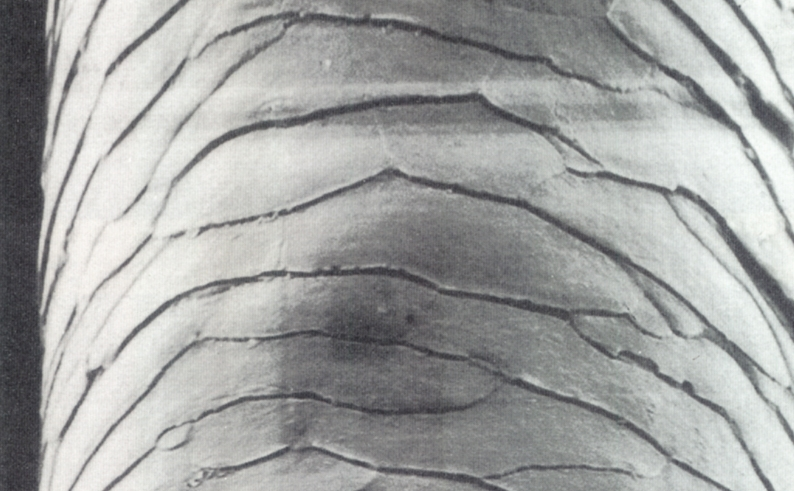
\includegraphics[scale=0.4]{images/hair_structure.jpeg}
\caption{The tilted cuticle scales on the outside of the hair fiber.}
\label{fig_hair_structure}
\end{center}
\end{figure}



\section{Rendering hair}

Marschner et al.~\cite{marschner} explain that hair rendering is a complex task, because local and global properties of hair must be taken into account. Local properties describe how light interacts with hair fibers and global properties describe the propagation of light through a volume of hair. In general, hair can be modelled explicitly or implicitly.

\subsection{Explicit Representation}

Hair research began by analyzing hair models using an explicit representation. This means that a hair model is represented as individual strands, or one-dimensional curves in three-dimensional space. Building on these foundations, researchers tried to find an efficient model to render a full head of human hair. Though several paths have been followed, modelling a full head of hair remains a challenge due to the geometric complexity and the thin nature of an individual strand coupled with the complex scattering effects and shadows that occur among the hairs~\cite{ward}.

\subsection{Implicit Representation}

Implicit hair representations stay away from the complexities of individual strands. With implicit representations, hair is rendered by approximating the appearance of the several strands using simpler and more efficient rendering strategies. Voxel grids, multi-layer textures or polygonal boundary representations are some of the possibilities to efficiently render a full hair model.

Implicit hair is usually modelled as a volume or polygonal boundary representation. Implicit representations work great when looking at hair from a distance, because at a distance the detail is hardly visible. Moreover, it is much faster in rendering and still giving good-looking results.

%Kajiya and Von Herzen [] suggested that volume densities were potentially capable of rendering hair and furry surfaces. Kay et al [] tried to implement this via three dimensional array of parameters. This means that a voxel cell can be maintained that holds data for each cell describing the average properties of the objects existing in this voxel cell.
%A hair density function can then be used to determine where the hair strands are and what the 

%Hair fibers cast shadows onto each other and they also receive or cast shadows on other objects in the scene. Self-shadowing is very important to render realistic looking hair. Without it may result in flat images. In general, there are two rendering strategies to incorporate self-shadowing in hair: ray casting through volumetric densities and shadow maps.



%Different known implicit representation

%Volumetric textures (or texels) [61], [62] avoid the aliasing problem with prefiltered shading functions [survey on hair modeling].



The downside of implicit representations is that it is not physically based and it is not flexible. Local scattering behaviour such as reflection and refraction, based on viewing direction and orientation of the hair strand are simplified. For physically based rendering, the explicit representation is the only way to go.

\subsection{Geometric complexity}

A human scalp may consist of over 200.000 hair strands. Some animals, such as bears might realistically be rendered with millions of hair strands. It is clear that the amount of hair fibers lead to a geometric complex challenge. 

A hair fiber is naturally represented with a curved cylinder. A single hair fiber can be represented in different ways. Connected triangle strips facing the camera may be used. Triangles are easy to intersect and a strip that always faces the camera will always be intersectable.

Another strategy is to extend camera facing triangle strips, making three ribbons and attach the ends together to form a trigonal prism.

Another strategy is to make use of a cylindrical primitive. This is the most realistic solution, since hair fibers are it comes closest to how a hair fiber is physically represented. Normals are also straightforwardly find when ray-tracing a cylinder.

In this project a single hair fiber is represented  as a one-dimensional curve in three-dimensional space. When rendering these curves are used to make a camera facing triangle strip to be able to ray-trace the curve.

\subsection{Aliasing problem}

A hair fiber is extremely thin. It is usually much smaller than the size of a pixel. Tracing a ray through a pixel will most likely miss the hair fiber.  To be able to render a hair strand is challenging and introduces aliasing. 

According to Hadap et al.~\cite{hadap} There are in general two strategies to perform anti-aliasing:

\begin{itemize}
\item Oversampling: With oversampling you cast a lot of rays through a single pixel so that enough rays hit the fiber to smooth out the aliasing effect. This is a very expensive solution, because it increases rendering time considerably For example, tracing 128 samples through a pixel could lead to a 128 times higher rendering time.

%First the hair fiber is projected onto the view plane. This makes it possible to accurately determine what pixels are affected by the hair fibers. By doing this for all hair fibers, we know exactly which hair fiber contributes to a certain pixel. By sorting the hair fibers for each pixel from front to back, we know what hair strand is before the other. The thing that needs 

%This results in point locations on the view plane. These points describe the exact location where the hair fiber is  Now we know what pixels are affected and their accurate positions inside the pixel.

\item Pixel Blending: blend the contribution of each hair fiber per pixel. This comes close to rasterization. Assuming that a curve is represented as a one-dimensional curve in three-dimensional space, then a fiber consists of a sequence of curve points. Drawing a spline based on these curve points, one can compute the contribution at each fragment of the curve, then backprojecting on the camera plane to find out which pixel is affected and add the contribution to the pixel. Blending needs to be performed to incorporate fibers that are positioned behind each other.

\end{itemize}

Physically based rendering is based on ray-tracing, so in this project the aliasing problem is overcome by oversampling and by giving each hair fiber a certain width when rendering. Increasing the width of a hair fiber makes it easier to ray-trace, thereby reducing the need for many samples. The Renderman Shading Language (RSL) has built in functionality to render curves. 

\subsection{Mathematical Notation}

The notation that is used in this thesis is the same as the one used by Marschner et al.~\cite{marschner} and is common in the field of hair rendering. A hair strand is represented as a one-dimensional curve in three-dimensional space. A $uvw$ coordinate axis is attached to any point along the curve.

The $u$-axis is tangent to the hair fiber and pointing in the direction from the root toward the tip. $v$ and $w$ complete a right-handed orthonormal basis and are situated in the normal plane of the hair fiber. If the cross section is elliptical, then  $v$ represents the major axis and $w$ the minor axis. The direction where the illumination is coming from is denoted by $\omega_i$ and the direction in which light is scattered is $\omega_r$. These directions are expressed in spherical angles $(\theta_i, \phi_i)$ and $(\theta_r,\phi_r)$ respectively.

The longitudinal inclinations with respect to the normal plane are denoted $\theta_i$ and $\theta_r$ and are measured so that $0\degree$ is perpendicular to the hair and $90\degree$ is $u$ and $-90\degree$ is $-u$. The azimuths around the hair are denoted $\phi_i$ and $\phi_r$, measured so that $v$ is $0\degree$ and $w$ is $+90\degree$.

Derived angles are used, such as the difference angle $\theta_d = (theta_r - \theta_i)/2$. The relative azimuth $\phi = \phi_r - \phi_i$. The half-angles are $\theta_h = (\theta_i + \theta_r)/2$ and $\phi_h = (\phi_i + \phi_r)/2$. Figure~\ref{axis_overview} shows an overview of the axes and spherical angles.

\begin{center}
\begin{figure}

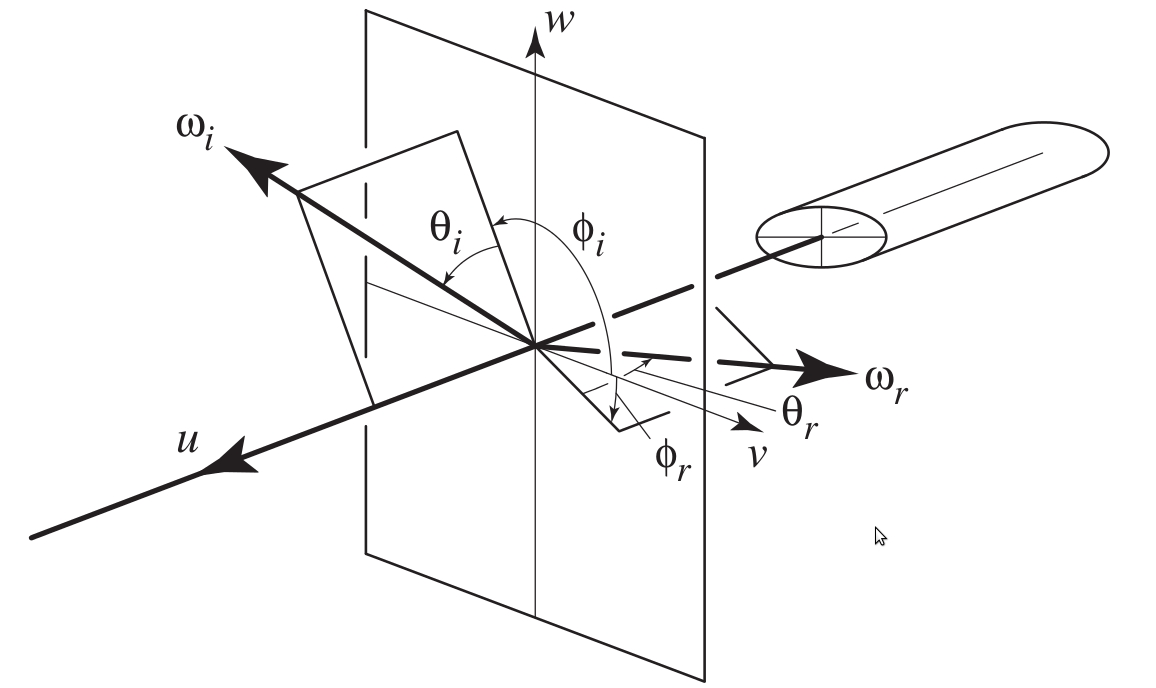
\includegraphics[scale=.4]{images/axes.jpeg}

\caption{An overview of the coordinate axes and the spherical angles with respect to a hair fiber. This is the convention used in this thesis and is used by Marschner et al. and most other hair rendering algorithms. Picture taken from Marschner et al.~\cite{marschner}.}
\label{axis_overview}

\end{figure}
\end{center}

\section{Radiometry}
It is important to understand the terminology in radiometry to get a good understanding of the theory that is explained in this report. If you are already familiar to this theory, you can skip this section. This theory is primarily meant for ones that are new to the field of rendering. 

\subsection{Power and radiant flux}

Power is the rate at which energy is transferred and is expressed in watts (W). A single watt describes the transfer of a single Joule (J) of energy per unit time (s).

A lot of electronic machines consume power, and each one does it in it's own particular way. You can think of light, heat, force, pressure, etcetera. Consider a light source that emits light particles through the scene at a certain rate. Some lights are stronger than others, meaning that the stronger light has more power and sends out the energy at a faster rate into the scene. These elementary light particles are called photons. Photons exhibit a wave-particle duality. On one side they can be treated as minuscule particles and on the other side they can be treated as waves, or more specifically: electromagnetic waves.

The rate at which a light source sends out electromagnetic waves is called radiant flux. Radiant flux $\Phi$ is the power of electromagnetic waves and describes the transfer of radiant energy (J) per unit time (s). Radiant flux is therefore also expressed in watts (W).

\subsection{Solid Angle and Radiant Intensity}

A two-dimensional angle can be thought of as drawing two lines from the center of a circle outward. Angles are represented as degrees or radians, but radians are more convenient for mathematical purposes. A solid angle $\Omega$ is the two-dimensional angle in three dimensional space that an object subtends at a point. Consider projecting a three-dimensional object onto a unit sphere. An object that is closer to the sphere may have the same solid angle as an object that is farther away. In this case, the object that is farther is bigger than the object closer to the unit sphere, but both have the same solid angle. A solid angle is a dimensionless unit of measurement called a steradian ($sr$). Steradian coming from squared radian.\\

The radiant intensity $I$ is a measure of the intensity of electromagnetic radiation. It can be seen as the energy flow divided by the solid angle in which it is transmitted. Radiant intensity is defined as radiant power per unit solid angle ($W \cdot sr^{-1}$).

\subsection{Radiance versus Irradiance}
\label{radiance_irradiance}

Formally, irradiance $E$ is defined as the amount of power of electromagnetic radiation per unit area incident on a surface. The unit for irradiance is watts per square meter ($W \cdot m^{-2}$). 

Radiance $L$ measures the light intensity per unit area on a surface. It measures the quantity of radiation that passes through or is emitted from a surface and falls within a given solid angle in a specified direction. Radiance is used to characterize diffuse emission. The unit of radiance is watts per steradian per square meter ($W \cdot {sr}^{-1} \cdot m^{-2}$).

\begin{equation}
L = \frac{d^2 \Phi}{dA\, d\Omega\, \cos \theta} \approx \frac{\Phi}{\Omega A \cos \theta}
\end{equation}

Figure~\ref{cosine_term_visualization} shows a simplified scenario of the sun shining on a surface. Irradiance is the amount of flux that is received per unit area, or in other words, the amount of sunshine impinging on the surface divided by the surface area. If we consider a rectangular bundle of light that hits the surface from a perpendicular direction $\omega_i$, then it is obvious to see that all the light falls into an equally sized rectangle on the surface. The irradiance would be equal to the power (or wattage) of this bundle of light, divided by the surface area, assuming this is the only light that shines on the surface.

As the sun moves along the sky, the direction from which it hits the surface changes. At some point, the sunlight is coming from a more glancing direction $\omega_i'$. If we consider the same rectangular bundle of light with size $w$, we notice that this bundle of light now spreads its power over a larger area. A larger area means that the irradiance becomes smaller. The same rectangular surface area does not receive the full potential power of the bundle of light anymore.

As the sun goes down, a point will eventually be reached that the direction of the sun rays will be parallel to the surface (or perpendicular to the surface normal $n^\rightarrow$). In this case none of the sunlight is able to reach the surface anymore.

In reality, the irradiance is computed for an infinitisemal small area $dA$. If the area becomes infinitisemal small, the irradiance from direction $\omega_i$ becomes a infinitisemal small bundles as well. Therefore in a bidirectional reflection distribution function (BRDF) the irradiance is sampled for a single direction.


\begin{figure}[h]
\begin{center}
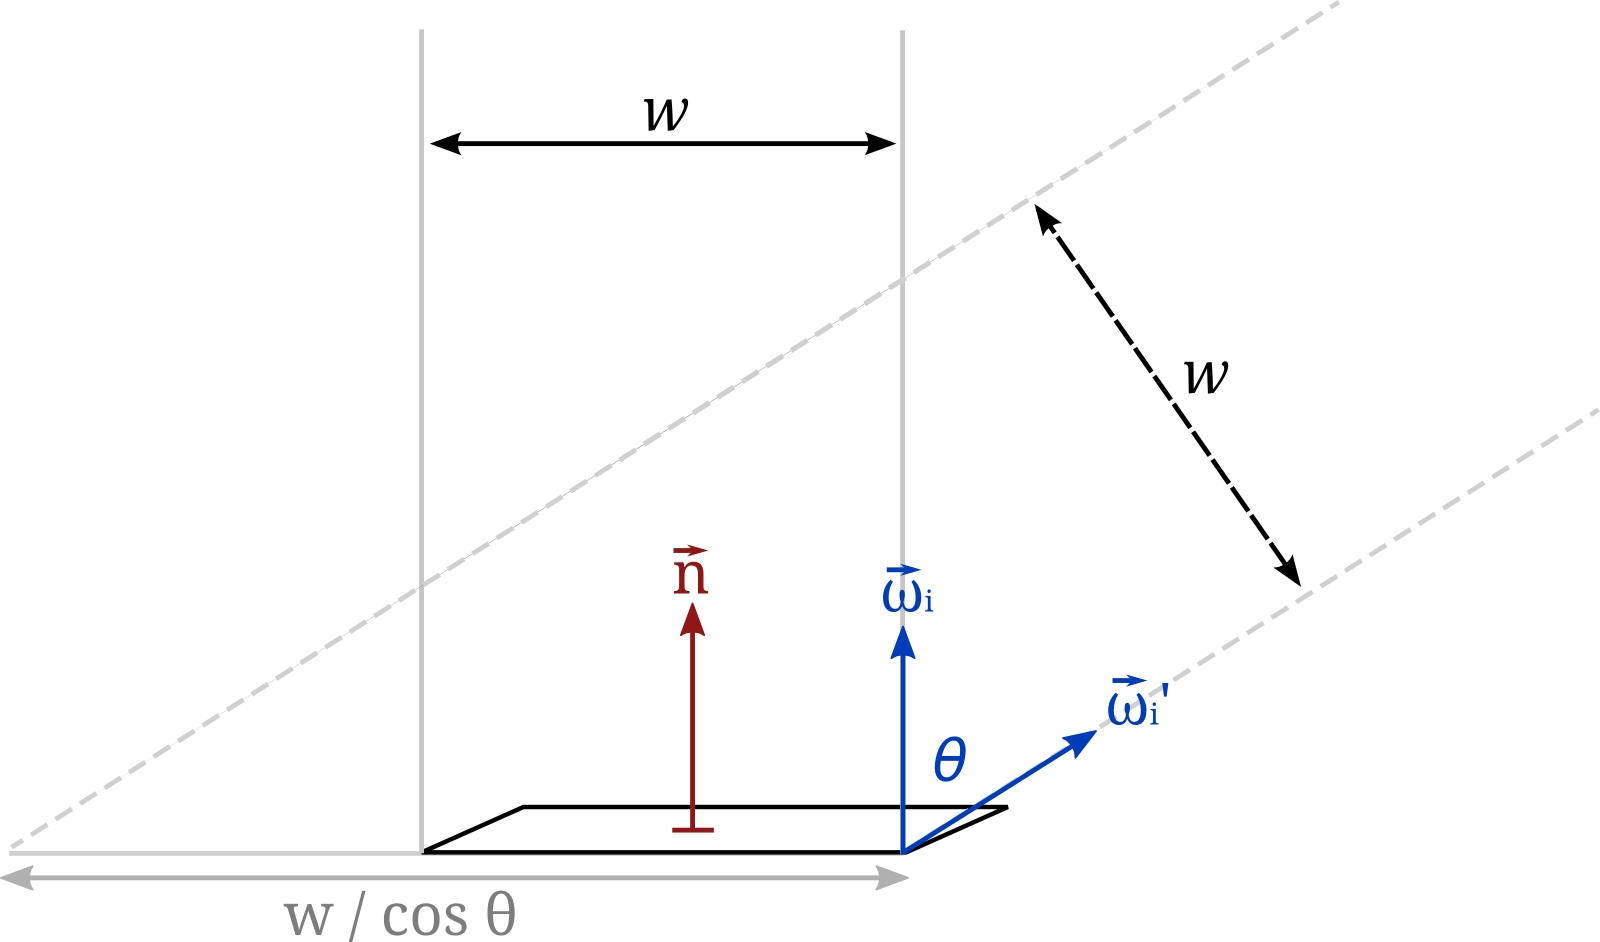
\includegraphics[scale=1.4]{images/svg/irradiance_radiance.jpg}
\caption{As the incoming light hits the surface at a larger angle, the irradiance decreases because the same amount of light will be spread over a greater surface area.}
\label{cosine_term_visualization}
\end{center}
\end{figure}


\subsection{Bidirectional Reflection Distribution Function (BRDF)}

When a surface is lit by a light source, part of it will scatter back into the environment. The distribution at which light is scattered back can be described by a bidirectional scattering distribution function (BSDF). If the surface is opaque and we are only taking into accounts reflection inside the hemisphere, then the reflection behaviour can be described by a bidirectional reflectance distribution function (BRDF). At some point $p$ on the surface, the BRDF function $f_r$ describes the relation between the amount of incoming radiance from direction $w_i$, $L_i(\omega_i)$, and the amount of reflected outgoing radiance in direction $w_o$, $L_o(\omega_o)$.

Physically based BRDFs have two important characteristics~\cite{pbrt}:

\begin{itemize}
\item Reciprocity: the incoming and outgoing directions can be swapped and still have the same reflection behaviour: $f_r(p, \omega_i, \omega_o) = f_r(p, \omega_o, \omega_i)$.
\item Energy conservation: the total amount of energy that is reflected will always be less or equal than the amount of energy that is incident on the surface.
\end{itemize}

Physically, a BRDF describes the relation between the amount of differentiated irradiance $dE(p, \omega_i)$ and the differentiated outgoing radiance $dL_o(p, \omega_o)$. 

\begin{equation}
f_r(p, \omega_o, \omega_i) = \frac{dL_o(p, \omega_o)}{dE(p,\omega_i)} = \frac{dL_o(p, \omega_o)}{L_i(p, \omega_i) \cos \theta_i d\omega_i}
\end{equation}

\subsection{Bidirectional Curve Scattering Distribution Function (BCDSF)}

Fibers are usually treated as one-dimensional curves. Therefore, scattering from fibers need to be described a little differently from the more familiar surface reflection~\cite{ward}. As discussed in the previous section, a BRDF describes the ratio between surface radiance exiting the surface in direction $\omega_r$, to surface irradiance falling on the surface from a differential solid angle $\omega_i$~\cite{ward}.

For fibers we are not talking about surfaces, but about lengths on a curve. This means that scattering from a fiber is described with a bidirectional curve scattering distribution function (BCSDF). A BCSDF describes the ratio between curve radiance exiting the curve in direction $\omega_r$ to curve irradiance falling on the surface from a differential solid angle $\omega_i$. It shares the same physical units, but the concept is a little different.

\begin{equation}
S(\omega_i, \omega_r) = \frac{dL_r(\omega_r)}{dE_i(\omega_i)}
\end{equation}

$L_r$ is the curve radiance scattered from an infinitesimal length of fiber and $E_i$ is curve irradiance on that portion of the fiber~\cite{marschner}. Curve irradiance is proportional to incoming curve radiance:

\begin{equation}
dE_i(\omega_i) = D L_i(\omega_i) \cos \theta_i d \omega_i
\end{equation}

Here $D$ denotes the diameter of the fiber. So, curve irradiance is the amount of light falling on an infinitesimal small length of curve $dl$, times the diameter of the fiber: $D dl$. Using the former equation, the scattering integral can be written as:

\begin{equation}
L_r(\omega_r) = D \int S(\omega_i, \omega_r) L_i(\omega_i) \cos \theta_i d \omega_i
\end{equation}


\subsection{Rendering Equation}
The rendering equation is an integral and formally describes the amount radiance leaving from a position $p$ in direction $\omega_o$. The radiance consists of the emitted light $L_e$ plus the integral around the sphere to integrate all incoming light $L_i$ from incident direction $\omega_i$, reflecting in direction $\omega_o$, where the BSDF is denoted by $f(p, \omega_o, \omega_i)$ indicating the contribution of incident light reflected in the outgoing direction at position $p$. The cosine factor is to take into account the angle with the surface (see section~\ref{radiance_irradiance}).

\begin{equation}
L_o(p, \omega_o) = L_e(p, \omega_o) + \int_{\Omega} f(p, \omega_o, \omega_i)\, L_i(p, \omega_i)\, \cos \theta_i\, d\omega_i
\end{equation}

Solving this equation is the key task for a computer graphics program. Hair fibers do not emit radiance and therefore the emitted radiance can be ignored in the rendering equation, obtaining the following equation that will be used in this thesis.

\begin{equation}
L_o(p, \omega_o) = L_e(p, \omega_o) + \int_{\Omega} f(p, \omega_o, \omega_i)\, L_i(p, \omega_i)\, \cos \theta_i\, d\omega_i
\label{renderingEquation}
\end{equation}

%
% ===============================================================================
%  Importance sampling
% ===============================================================================
%

\section{Importance Sampling}
\label{basics_importance_sampling}

% The need for importance sampling

Importance sampling is a variance reduction technique. The idea is to prefer samples that have more impact on the end result (i.e. the rendering) than samples that hardly have an influence. In other words, samples with a higher impact are more important to sample from, than samples that hardly have impact. By prefering samples of important directions we are converging faster to the correct end result, thereby decreasing rendering times significantly.

\subsection{Monte-Carlo integration}
% Introduction to monte-carlo integration 

Given a function $f(x)$ that we want to integrate over the range $[a, b]$. Determining the integral can be done in numerous ways. If it is possible to find the integral equation for $\int f(x) dx = F(x)$, then we could solve the integral analytically and there would be no need for Monte-Carlo integration.

In the context of physically based rendering, the integral is often too complicated to solve analytically. The Monte-Carlo integration is a relatively simple way to be able to find the expected value of an integral. Monte-Carlo integration is doing that by taking $N$ random samples and averaging the result, thereby coming closer to the correct result. The larger the number of samples, the more accurate the result will be, eventually converging to the correct result for the integral.  The following equation describes the computation of the integral $F_N$ with the Monte-Carlo estimator~\ref{pbrtbook}.

\begin{equation}
F_N = \frac{1}{N} \sum_{i=1}^{N} \frac{f(X_i)}{p(X_i)}
\end{equation}

$N$ represents the number of samples taken, $X_i$ represents the $i$-th random sample and $p(X_i)$ is the probability density for sample $X_i$. If the probability density function $p(x)$ is constant, the equation becomes finding the average value and then multiplying by the size of the domain.

\subsection{Importance sampling}
\label{section_importance_sampling}
% Adding importance sampling to the fact

It becomes interesting when the probability density function $p(x)$ is not constant for all samples. By giving certain samples a higher probability and other (less important) samples a lower probability, we can converge faster to the correct result by using less samples.

The idea behind importance sampling is to draw samples from the probability distribution function (PDF). There are different techniques to draw samples from a PDF as explained in the book by Pharr et al.~\ref{pbrtbook}. Possible techniques are inversion sampling, in which the normalized cumulative distribution function (CDF) is computed, then inverted and used with a uniform random variable $\Xi \in (0, 1]$ to obtain a sample $X$. Other techniques are rejection sampling.
 
It is easy to see that the better the fit of the PDF with the function $f(x)$, the better the drawn samples and the faster we converge to the correct result. If $f(x) = p(x)$ we are talking about perfect importance sampling, the most ideal case. However, it is not always possible to invert $f(x)$. If we can find a PDF that is still a close fit to $f(x)$ but is possible to invert, then we still have a better sampling technique compared to uniform sampling.

Other techniques are possible as well, such as rejection sampling, which is described indetail in Pharr et al.~\ref{pbrtbook}.

\subsection{Multiple importance sampling}
% Multiple importance sampling

Sometimes we end up with a function that can be written as the product of multiple functions $f(x)g(x)$, each of which has an easy to sample from PDF $p_f(x)$, belonging to $f(x)$ and $p_g(x)$ for $g(x)$.

If two sampling distributions $p_f(x)$ and $p_g(x)$ are used to estimate the value of $\int f(x)g(x) dx$, you cannot just average the results by taking N samples from $p_f(x)$ and M samples from $p_g(x)$ and average the result, because variance is additive. The way how to do it is by using the new Monte-Carlo estimator for multiple importance sampling (MIS) stated in~\ref{pbrtbook}: 

\begin{equation}
\frac{1}{n_f} \sum_{i=1}^{n_f} \frac{f(X_i)g(X_i) w_f(X_i)}{p_f(X_i)} + 
\frac{1}{n_g} \sum_{j=1}^{n_g} \frac{f(Y_j)g(Y_j) w_g(Y_j)}{p_g(Y_j)} 
\end{equation}

where $w_f$ and $w_g$ are weighting functions.

\begin{equation}
w_s(x) = \frac{n_sp_s(x)}{\sum_i n_i p_i(x)}
\end{equation}




\chapter{Related Work}

% a. Discuss the existing methods and state why they cannot solve the problems or achieve the goal entirely.
% b. Discuss other related work or knowledge that is necessary to understand the theory explained in Chapter 3.
% c. Ask yourself if the information will be sufficient if a student who is new in the field reads this chapter.





\section{Hair Rendering Overview}

The explicit representation of hair provides the most physically accurate results, because simulating the scattering events fiber by fiber is also what happens in nature. Considering a single hair fiber, models have been proposed to render such a fiber. To increase the realistic appearance of hair fibers, more fibers should be taken into account. This leads to the concept of multiple fiber scattering. Multiple fiber scattering is analogous to subsurface scattering in solid materials and therefore necessary to increase the level of realism. Ward et al.~\cite{ward} provides a good overview on the different models in hair rendering in general.

In this section, related work regarding the development of hair models is explained, followed by an in-depth treatment of the most relevant work related to the research in this paper.


\subsection{Single fiber scattering}

Kajiya and Kay~\cite{kajiya} provided one of the first widely used hair scattering model that was designed to render fur. Fur usually refers to a  dense coat of fine and soft hair. Their idea was that fine hair geometry should not be represented with complex geometry which leads to aliasing effects, but with texels. A texel is a three-dimensional texture map intended to represent a highly complex collection of surfaces contained within a defined volume~\cite{kajiya}.

The rendering of the hair model was based on a diffuse and specular component. The diffuse component is obtained by simply integrating a Lambert surface along one half of the cylinder facing the light source. The specular component is based on the Phong model in which light is reflected at a mirror angle along the tangent. Since the normals on the cylinder point in directions perpendicular to the tangent, the reflected light forms a cone whose angle at the apex is equal to the angle of incidence~\cite{kajiya}. The Kajiya and Kay model is clearly an ad-hoc model where hair fibers are treated as opaque cylinders, limiting the realism of the model.\\

The Kajiya and Kay model lacks directionality, meaning that hairs are fully lit independent on the light direction or eye position. Goldman~\cite{goldman} was interested in reflection and transmission and increased directionality by introducing two new attenuation factors. These attenuation factors can be used to tune the relative transmissivity and reflectivity of a hair. It does this by computing a value $f_{\textsc{dir}}$ that is multiplied with the contribution of the Kajiya and Kay model.\\

Marschner et al.~\cite{marschner} improved the Kajiya and Kay model substantially by proposing the most physically based hair scattering model at that time. Their model makes two improvements to Kajiya and Kay's model: it predicts the azimuthal variation in scattered light based on the ray optics of a cylinder, and it accounts for the longitudinal separation of the highlight into surface-reflection, transmission, and internal-reflection components that emerge at different angles~\cite{hadap}. The Marschner model is described in detail in section~\ref{sec_marschner}.


\subsection{Multiple fiber scattering}

For fully realistic results, light that reflects from hair to hair, or multiple scattering, must be accounted for~\cite{ward}.

Multiple fiber scattering extends single fiber scattering to include the scattering effects between seperate hair strands. A single fiber scattering model can be used as the basis for multiple fiber scattering. For example, if the Marschner model is used for single fiber scattering in combination with path tracing along all the hairs in hair model, we obtain the result for multiple fiber scattering. Path tracing is realistic, but given the geometric complexity of a hair model, a very time consuming process. More efficient multiple fiber scattering models should be devised.\\

Photon mapping methods can reduce per-frame rendering times from days, required for path tracing methods, to hours~\cite{ward}. Photon mapping is a practical approach for computing global illumination in complex environments. Photon mapping is introduced by Henrik Wann Jensen~\cite{jensen} and it is, in general, a two-step approach.
The first pass in the method is constructing the photon map by emitting photons from the light sources in the model and storing these in the photon map as they hit surfaces~\cite{jensen}. The collection of photons distributed in the photon map, can be seen as a rough representation for the amount of light in the scene. The second step is that this information from the photon map is used to render the scene.

For multiple scattering in hair models, Moon and Marschner~\cite{moon} developed a model using a photon mapping approach. In the first pass, particles are traced from light sources into the hair volume and followed through multiple scattering events, and their positions and directions are stored into a 5D hierarchical data structure to record the flow of particles through space~\cite{moon}. In the second pass a density estimate is performed simultaneously in position and direction to estimate the radiance arriving at a hair from a particular direction.  This photon mapping approach leads to similar results compared to path tracing, but the biggest drawback is that it requires high resolution photon maps (memory usage) and the method is not interactive.

The Dual Scattering approximation is a direct extension on top of Marschner and doesn´t have the drawbacks of photon mapping approaches. The dual scattering approximation splits up the compensation in a global and a local scattering component. The global scattering component computes the amount of irradiance reaching a certain position in the hair model. The local scattering component uses the computed irradiance to compute the scattering effects in the direct neighbourhood of the position to be rendered. More in-depth theory is provided in section~\ref{sec_dualscattering}.

%
% ===============================================================================
%  Marschner Model
% ===============================================================================
%

\section{Marschner model}
\label{sec_marschner}
%
% Goal of Marschner 
%

The biggest drawback of Kajiya and Kay~\cite{kajiya} is that their scattering model is not based on physical measurements. Instead, it uses a simple ad-hoc term with a constant linear highlight. Marschner et al. ~\cite{marschner} proposed a physically based scattering model for single fiber scattering. The single fiber scattering model, or Marschner model, forms the basis for the dual scattering approximation and will be discussed in detail.


\subsection{Observations}
%
% Basic observation
%
 
In order to come up with a physically based scattering model for single hair fibers, Marschner et al. devised a setup to capture the response of light scattered against a hair fiber. 

They illuminated individual hairs with a narrow beam and measured the scattered light in various directions, using a setup based on a four-axis goniometer that positioned a light source and a CCD camera at arbitrary directions from the sample~\cite{marschner}. Their measurements show a couple of distinct characteristics for human hair.

\subsubsection{Longitudinal variation}
\label{sec_longitudinal_observation}

Stamm et al. and Bustard and Smith measured the scattering behaviour in the incidence plane. This is the 2D slice for which the hair fiber is coplanar with the source and detector. Marschner et al. did the same measurements and placed a light source under a direction of positive and negative 45 degrees with the hair fiber ($\theta_i = +/- 45\degree$). See figure~\ref{fig_longitudinal_marschner} for the measured responses.

Observations show that synthetic hair has a highlight that appears exactly at the specular direction ($\theta_r = -\theta_i$), but for real hair fibers the specular highlight is shifted toward the root of the hair fiber. This is due to the tilted cuticle scales that have a surface orientation that is shifted by approximately 6 to 8 degrees from the ideal cylinder surface normal. This highlight is the result of scattering against the surface of the hair fiber. It is called the primary specular highlight and appears as having the color of the light source.

\begin{figure}[h]
\begin{center}
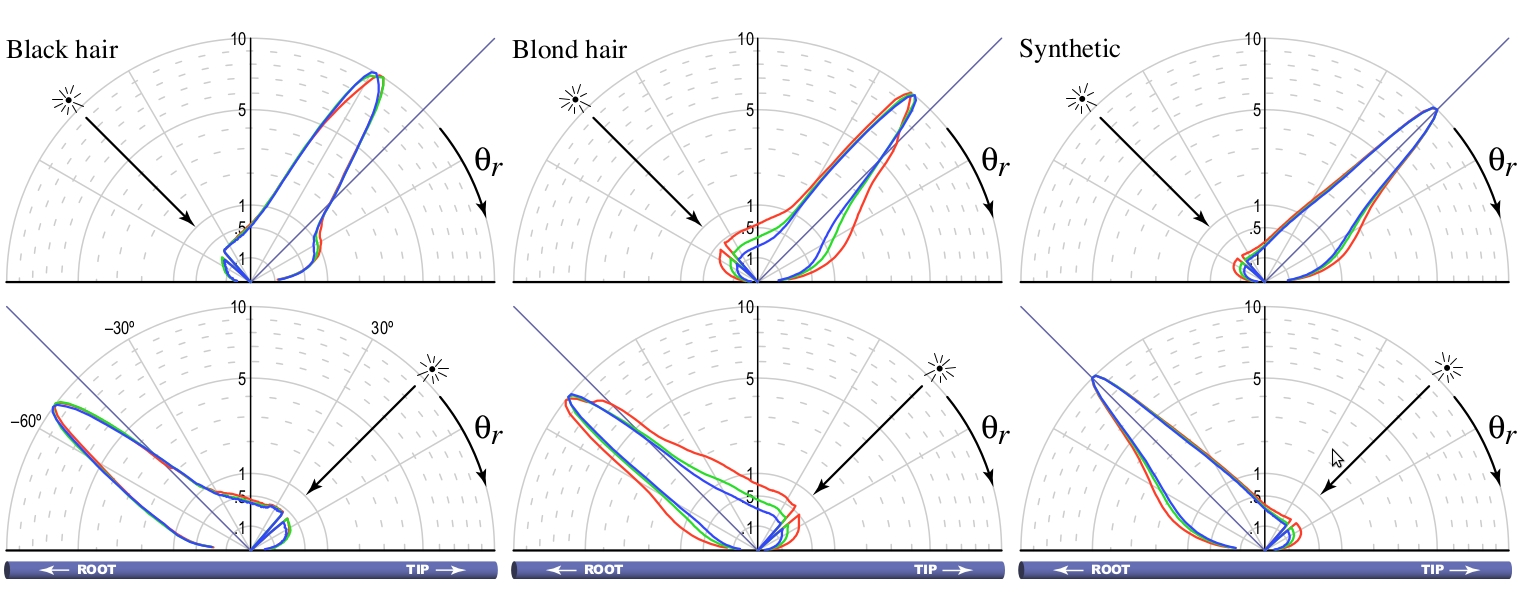
\includegraphics[scale=0.35]{images/longitudinal_response.jpeg}
\caption{The scattering behaviour in the incidence plane (longitudinal scattering). For human hair the specular reflection is shifted towards the root by a few degrees. For synthetic hair no shifted highlight is visible, because synthetic hair doesn't consist of tilted cuticle scales.}
\label{fig_longitudinal_marschner}
\end{center}
\end{figure}

Another observation is that blond hair has a coloured secondary peak. This can be seen by the red response that is slightly higher compared to the blue and red response. The secondary peak can be explained by internal scattering. Consider the hair fiber as a cylinder; when light enters the cylinder, the light will first refract, then propagates through the core of the fiber and bounces back against the other end of the fiber. When leaving the fiber, the light refracts again. This reflection and refraction behaviour causes the deviation from the primary specular highlight. During its travel, light propagated through the center of the hair fiber, where the pigments are. These pigments absorb part of the energy in different wavelengths. This is how the secondary peak gets its colour.

Furthermore, Marschner et al.~\cite{marschner} noted that as the scattering angle increases, the secondary highlight fades out, while the primary highlight maintains more constant amplitude. Both peaks maintain approximately constant width and at high angles the primary highlight becomes a sharp peak that is prominent very close to the specular direction. 


\subsubsection{Azimuthal variation}


\begin{figure}[h]
\begin{center}
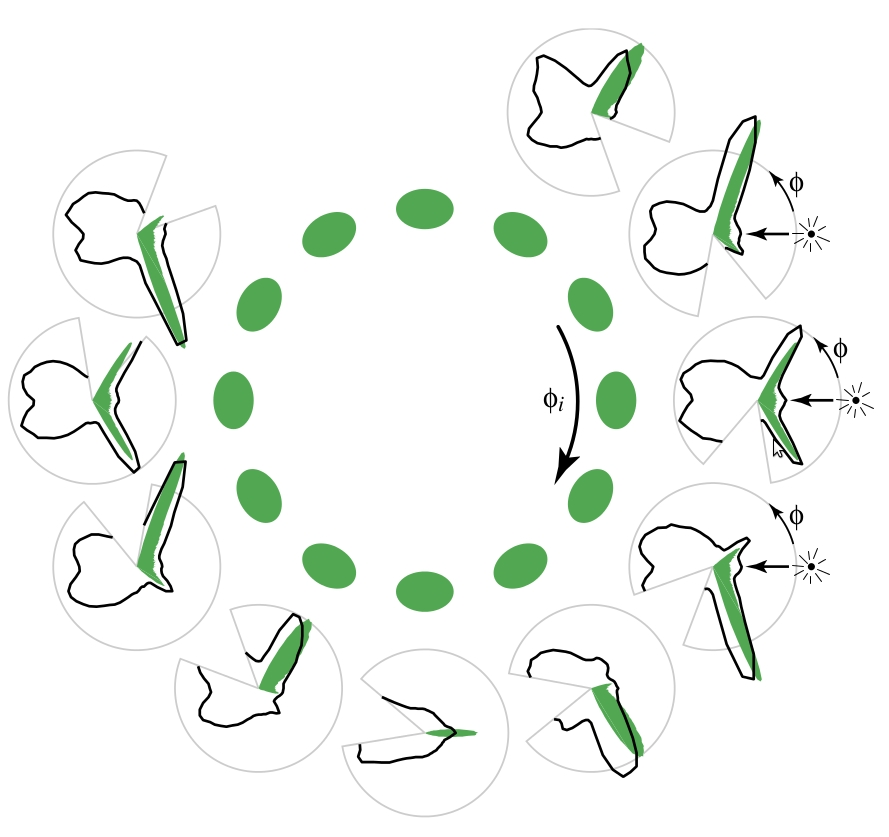
\includegraphics[scale=0.4]{images/azimuthal_measurement.jpeg}
\caption{Measurements of azimuthal scattering (scattering in the normal plane). The light source is shining from the right, while the hair fiber is rotated. The green ellipse is the cross section of the fiber for different measurements with increasing rotations of the fiber. Figure taken from Marschner et al.~\cite{marschner}.}
\label{fig_azimuthal_marschner}
\end{center}
\end{figure}


Azimuthal variation is measured by placing the light and detector in the plane that is perpendicular to the hair fiber: the normal plane. In figure~\ref{fig_azimuthal_marschner} plots are displayed that show the azimuthal scattering response with varying $\phi_i$ and $\phi_r$. The setup is that the light source is fixed (targeted from right to left) and the hair fiber is rotated. 

In this normal plane setup, it is clearly visible that there are two bright out-of-plane peaks. Out of plane, because the response is captured at $\theta_r = 10$ degrees, due to the tilted cuticle scales discussed before. These peaks are called glints.

The glints change considerably in brightness and position as a function of $\theta_i$,  meaning that the hair is not rotationally symmetric~\cite{marschner}. This is because the hair is eccentric and has an elliptical cross section. More generally, the evolution of the peaks as the fiber rotates appears similar to the internal reflection from a transparent elliptical cylinder~\cite{marschner}.

Figure~\ref{fig_azimuthal_marschner} also shows a strong transmission component. This is light that passes through the hair fiber and leaving on the other side of the fiber as seen from the light source. This means that the Marschner hair model takes three scattering modes into account. R stands for reflection and T for transmission:

\begin{itemize}
\item R: Specular reflection that is deviated slightly from the perfect specular direction, due to the cuticle scales.
\item TT: Transmission component that enters the fiber, propagates through it and leaves the fiber at the other end.
\item TRT: Internal reflection, that enters the fiber, scatters back and leaves again at the same side as where it entered.
\end{itemize}

More scattering modes are possible as well, such as TRRT or TRRRT. These events are ignored, because their contributions become negligible small due to loss of energy after that many reflection events. Instead, Marschner et al.~\cite{marschner} suggests to add a little diffuse color for better looking results. In figure~\ref{female_hair} an image is shown with the three scattering components clearly visible.

\begin{figure}[h]
\begin{center}
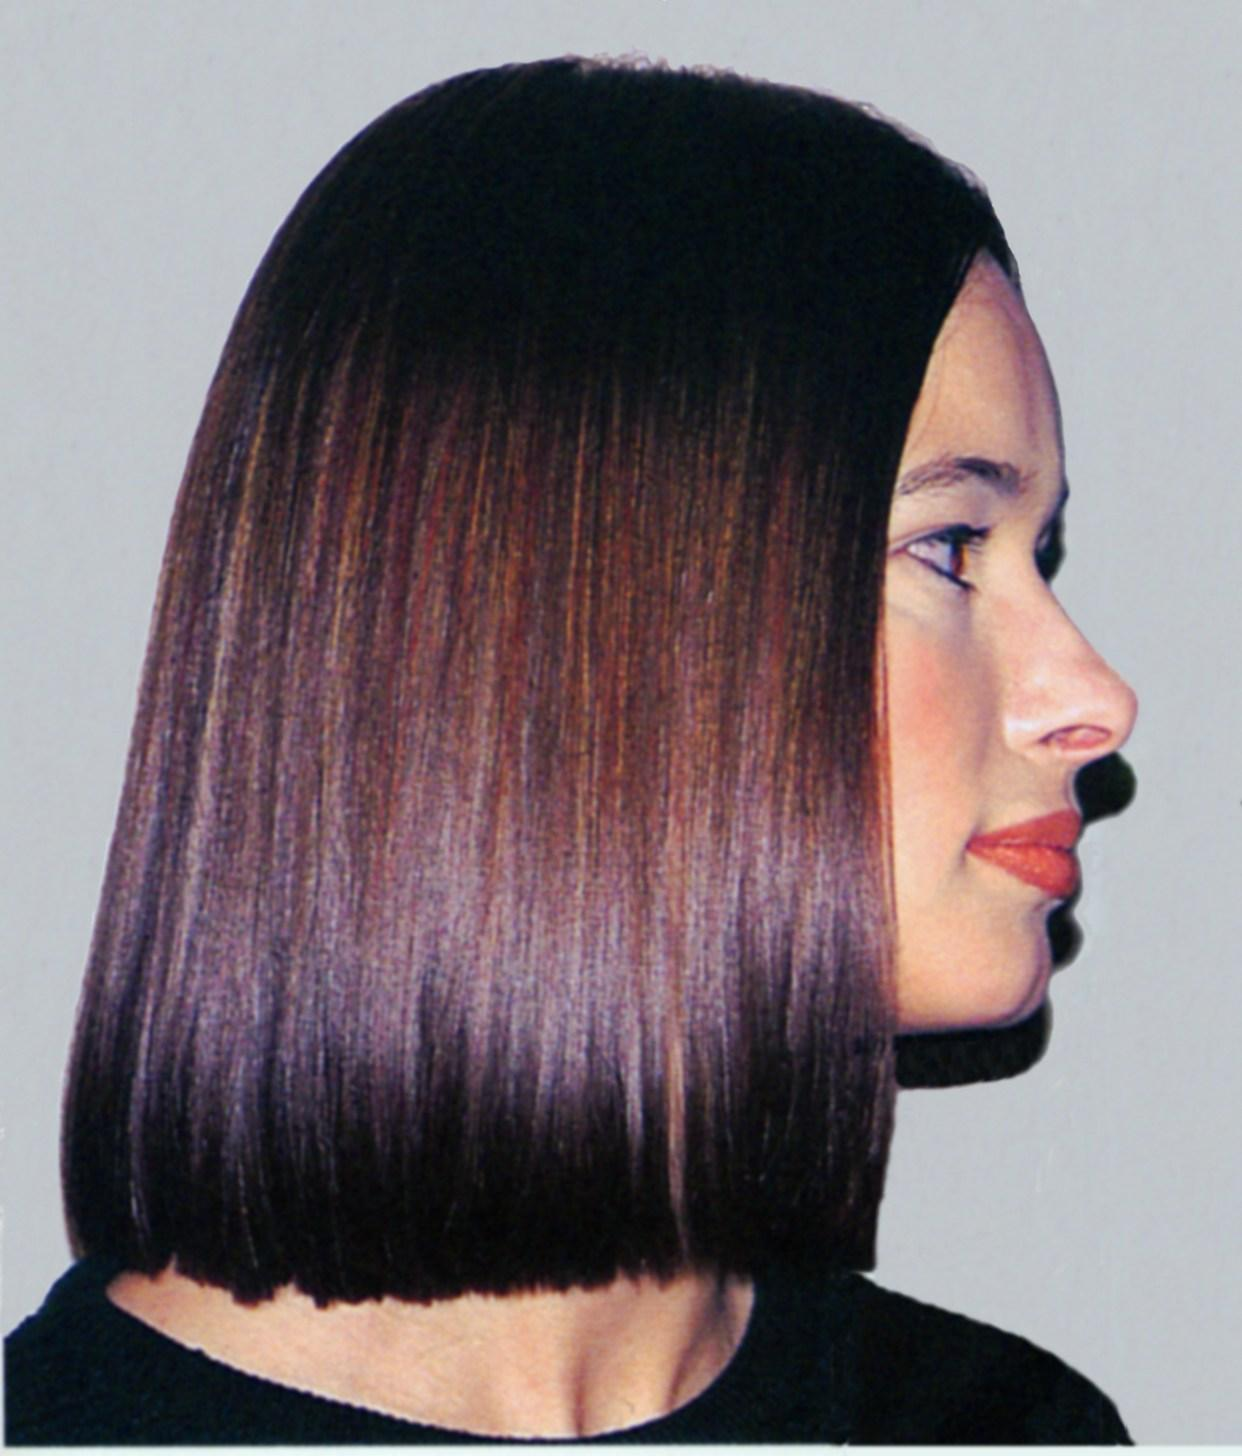
\includegraphics[scale=0.2]{images/female_marschner.jpeg}
\caption{An image from Gray~\cite{gray} showing a female with brown hair. The three scattering modes: R, TT and TRT contributions are visible in the hair. Glints give hair it's characteristic texture.}
\label{female_hair}
\end{center}
\end{figure}

\subsection{Model}

There are properties that have been used in previous work on scattering from fibers ([Marcuse 1974; Adler et al. 1998; Mount et al. 1998]):

\begin{itemize}
\item A ray that enters a dielectric cylinder at a particular angle to the axis will always exit at the same angle, regardless of the sequence of reflections and refractions it undergoes.

\item The dependence of the scattered distribution can be analysed by examining only the projection into a plane perpendicular to the hair.
\end{itemize}

Based on the observations described in the previous subsection and the theory here, Marschner et al. came up with a model that is divided into a longitudinal scattering function $M_p$ and an azimuthal scattering function $N_p$, where $p$ is the scattering mode with $p \in \{\textnormal{R}, \textnormal{TT}, \textnormal{TRT}\}$. The resulting scattering model can then be noted as:

\begin{equation}
\label{marschner_model_scatterfunction}
S(\omega_i, \omega_r) = \frac{\sum_{p \in \{\textnormal{R}, \textnormal{TT}, \textnormal{TRT}\}} M_p(\theta_i, \theta_r) N_p(\eta'(\theta_d); \phi_i, \phi_r)}{\cos^2 \theta_d}
\end{equation}

$S$ depends on incoming and outgoing angles $\omega_i$ and $\omega_r$, but can be reduced to a 2D scattering function, since the scattering model makes use of the difference angles $\theta_h$ and $\phi$.

\subsubsection{Longitudinal Scattering Function}
\label{marschner_longitudinal_scattering_function}

Using the first property of scattering from fibers, it can be derived that the angle of incidence is the same as the angle of reflection ($\theta_i = -\theta_r$). There are two deviations that cause the reflection to not be exactly in the specular direction (see section~\ref{sec_longitudinal_observation}). First, the surface of hair fibers are rough, causing a spread of reflected light instead of a mirror like specular reflection. Secondly, the cuticle scales of the hair fiber are tilted, causing a 6 to 8 degrees deviation from the perfect specular direction.

Marschner et al. approximated the longitudinal scattering function $M$ by a unit-integral zero-mean Gaussian function $g(\beta, x)$, where $\beta$ equals the standard deviation and $\alpha$ equals the longitudinal shift. In a published paper by d'Eon et al.~\cite{eon2011}, they discovered that the Marschner model is not entirely energy conserving for several reasons. One of the reasons with most impact is that the use of the half angle $\theta_h$ instead of $\theta$ doubles the reflected energy on average. Additionally the Gaussian is normalized with respect to $\theta \in \{-\infty, \infty \}$, but is evaluated with $\theta_h \in \{ -\pi/2, \pi/2 \}$, thereby losing a considerable amount of energy when deflection happens for near grazing angles. The doubling of energy is easily accounted for by doubling the half angle in the Marschner longitudinal scattering function. The resulting longitudinal functions $M$ that are used for the Marschner model are thus as follows:

\begin{align}
M_{\textnormal{R}}(\theta_h) &= g(\beta_{\textnormal{R}}, 2\theta_h - \alpha_{\textnormal{R}}) \\
M_{\textnormal{TT}}(\theta_h) &= g(\beta_{\textnormal{TT}}, 2\theta_h - \alpha_{\textnormal{TT}}) \\
M_{\textnormal{TRT}}(\theta_h) &= g(\beta_{\textnormal{TRT}}, 2\theta_h - \alpha_{\textnormal{TRT}})
\end{align}

By varying the standard deviation $\beta$, the spread of the longitudinal scattering component can be adjusted to simulate the rough surface of hair fibers. $\alpha$ deviates the peak from the specular direction by shifting the gaussian distribution. Marschner et al~\cite{marschner} provided some typical values for $\alpha$ and $\beta$ (see table~\ref{table_marschner_alpha_beta}).

\begin{table}[h]
\begin{tabular}{c|l|c}
Parameter & Description & Typical value \\ \hline 
$\alpha_{R}$ & Longitudinal shift for R lobe & -10\textdegree\,to -5\textdegree \\
$\alpha_{TT}$ & Longitudinal shift for TT lobe & $-\alpha_R / 2$ \\
$\alpha_{TRT}$ & Longitudinal shift for TRTlobe & $-3\alpha_R / 2$ \\
$\beta_R$ & Longitudinal spread for R lobe & 5\textdegree\, to 10\textdegree\, \\
$\beta_{TT}$ & Longitudinal spread for TT lobe & $\beta_R / 2$ \\
$\beta_{TRT}$ & Longitudinal spread for TRT lobe & $2 \beta_R$ 
\end{tabular}

\caption{Typical values for parameters for the longitudinal scattering function. Taken from Marschner et al.~\cite{marschner}}
\label{table_marschner_alpha_beta}
\end{table}


\subsubsection{Azimuthal scattering Function}

The azimuthal scattering component requires more thought, since different scattering paths inside the circular cross section need to be considered. 

Scattering from a dielectric circle is well studied. Consider a parallel beam incident on a circular cross section at an offset $h$ from the center. A parallel beam incident on the center of a circle means that $h = 0$. A value of $h=+/-1$ indicates that the parallel beam is glancing the edges of the circle. Using the offset $h$, the angle of incidence $\gamma_i$ can be computed using the following equation:

\begin{eqnarray*}
\sin \gamma_i = h & \Leftrightarrow & \gamma_i = \arcsin h \\
\eta \sin \gamma_t = h & \Leftrightarrow & \gamma_t = (\arcsin h) / \eta
\end{eqnarray*}

A ray that is incident on the unit circle can be traced as it refracts and reflects through the circle. The exit angle is not only dependent on the incidence angle (or offset from the center), but also on the number of scattering events. The number of scattering events $p$ equals 1 for the reflection case, 2 for transmission (TT) and 3 for internal reflection (TRT). The exit angle can then be calculated as follows:

\begin{equation}
\label{eq_relative_azimuth_change}
\phi(p,h) = 2p \gamma_t - 2 \gamma_i + p \pi
\end{equation}

The figure from Marschner et al. provides a good overview on the possible scattering events and the relation between the scattering angles.

Consider rendering a scene using ray tracing and that a particular camera ray is incident on a hair fiber. To find the contribution for the rendered image, we need to find all the paths that contribute to scattering in the direction of the camera ray. These paths are found by solving for roots. The R and TT cases have exactly one root and TRT has either one or three roots. The $h$ values for these paths are found by solving for the roots of the function $\phi(p, h) - \phi = 0$. Finding the roots requires solving a cubic equation, which is explained deeper in Marschner et al.~\cite{marschner}. The roots are denoted by $h(p, r, \phi)$ where different values of $r$ denote different roots. \\


Attenuation has to be taken into account as well. Attenuation occurs because of reflections, refractions and absorption. The attenuation for reflections and refractions are computed using the Fresnel equation. The Fresnel equation takes a parallel and perpendicular index of refraction ($\eta'$ and $\eta''$ respectively). Absorption takes place when a ray propagates through the hair fiber. The length of each internal path segment is computed by applying the law of cosines. According to~\cite{}, the formula given in Marschner et al. is wrong. This equation should be as followed:

\begin{equation}
l = \frac{2r \cos \gamma_t}{\cos \theta_t}\,\,\, \textsf{with $\theta_t = -sgn(\theta_i) \arccos ((\eta'' / \eta') \cos \theta_i)$}
\end{equation}

Here $l$ denotes the length of a single internal path segment for the TT case. For TRT, the length doubles. $r$ is the radius of the hair fiber and is a setting provided by the user. Absorption is denoted by $T(\sigma_a, h)$ where $\sigma_a$ is the absorption coefficient. It describes the amount of absorption per unit length through the hair fiber. It follows straightforwardly that the absorption is computed as $T(\sigma_a, h) = \exp( \sigma_a l )$. The normal plane scattering function $N_p$ can now be described and is shown in equation~\ref{azimuthal_marschner} be described.

\begin{eqnarray*}
A(0, h) & = & \textrm{Fresnel}( \eta', \eta'', \gamma_i ) \\
A(p, h) & = & (1 - \textrm{Fresnel}( \eta', \eta'', \gamma_i ))^2 \cdot \textrm{Fresnel}( \frac{1}{\eta'}, \frac{1}{\eta''}, \gamma_t )^ {p-1} \cdot T(\sigma_a, h) \\
\label{azimuthal_marschner}
\end{eqnarray*}

The normal plane scattering function for a given number of path segments $p$ (1, 2 or 3) is given in equation~\ref{azimuthal_marschner}.

\begin{equation}
N_p(p, \phi) = \sum\limits_r A(p, h(p, r, \phi)) \cdot \Big \vert 2 \frac{d\phi}{dh}( p, h(p, r, \phi) ) \Big \vert^{-1}
\end{equation}

\subsubsection{Glints}

Because the theory is based on smooth surfaces, the normal plane scattering function $N_p$ for the TRT scenario produces singularities with infinite intensity~\cite{marschner}. These singularities are called caustics and is light that bundles together after a sequence of reflections and refractions. In reality, these caustics are bright spots of light that originate after a sequence of reflections and refractions. Think about light propagating through a wine glass for example. These infinite singularities are removed by replacing it with a smooth Gaussian lobe centered at the location of the caustic. This changes the normal plane scattering function for the TRT case. Marschner et al.\cite{marschner} provides more detail into how the scattering function changes.

\subsubsection{Taking into account eccentricity}

Changing refractive index has effects that are qualitatively similar to changing eccentricity~\cite{marschner}. In order to simulate eccentricity, the refractive index is computed based on the value of eccentricity $a$. The equation can be found below. More detail is in Marschner et al's paper~\cite{marschner}.

\begin{eqnarray}
\eta_1^* & = & 2(\eta - 1) a^2 - \eta + 2 \\
\eta_2^* & = & 2(\eta - 1) a^{-2} - \eta + 2 \\
\eta^*(\phi_h) & = & \frac{1}{2}\big((\eta_1^* + \eta_2^*)+\cos(2\phi_h)(\eta_1^* + \eta_2^*) \big)
\end{eqnarray}

\subsubsection{Marschner model}

From the description above we can now describe the complete Marschner scattering model $S(\omega_i, \omega_r)$.

\begin{eqnarray*}
S(\phi_i,\theta_i; \phi_r, \theta_r) & = & M_R(\theta_h) N_R(\phi) / \cos^2 \theta_d \\
& + & M_{TT}(\theta_h) N_{TT}(\phi) / \cos^2 \theta_d \\
& + & M_{TRT}(\theta_h) N_{TRT}(\phi) / \cos^2 \theta_d \\
\end{eqnarray*}

Here the longitudinal functions $N_x$ are placeholders for the normal plane scattering function $N_p$:

\begin{eqnarray*}
N_R(\phi) & = & N_p(0, \phi) \\
N_{TT}(\phi) & = & N_p(1, \phi) \\
N_{TRT}(\phi) & = & N_p(2, \phi) \\
\end{eqnarray*}
\subsection{Evaluation}

The advantage of the Marschner hair model is that it is based on physical observations. Compared to previous approaches this is a huge win. Finding the roots for a given direction is slow, but can be dealt with by using precomputed tables.

The Marschner hair model focuses on single fiber scattering and to render realistic hair volumes, multiple fiber scattering needs to be taken into account. Path tracing or photon mapping are possible approaches, but take a lot of time or require an extensive amount of memory. Another drawback is that from own calculations, the Marschner model is not energy conserving. Especially for very wide angles, the reflections will be relatively high.

%
% ===============================================================================
%  Dual Scattering
% ===============================================================================
%

\section{Dualscattering Approximation}
\label{sec_dualscattering}
%Summarize introduction

Multiple scattering is a key factor in the realistic rendering of hair, especially for dense light colored hair volumes (such as blond hair). The relative amount of absorption by light colored hair types is fairly low, so this means that light undergoes many scattering interactions inside the hair volume before the contribution is reduced to an amount that can be neglegible. The high geometric complexity of hair models coupled with the compexity of the light interaction in hair volumes makes computing the multiple scattering effect difficult~\cite{zinke}. Difficult to an extent that path-tracing is not a feasible solution, because it requires too much time and too many samples to reduce the noise and come to an acceptible rendering.

The dual scattering approximation, proposed by Zinke et al.~\cite{zinke} splits the multiple scattering computation in two components: global multiple scattering and local multiple scattering. The global multiple scattering component aims to compute the light traveling through the hair volume and reaching the neighborhood of the point of interest, while local multiple scattering accounts for the scattering events within this neighborhood~\cite{zinke}.

%
%Start from general rendering equation
%

Starting from the general rendering equation
%~\ref{\label{renderingEquation}}
and ignoring the position component in the BSDF description as is common for material definitions, because materials usually behave the same irrespective of position, we obtain the following equation.

\begin{equation}
L_o(x, \omega_o) = \int_{\Omega} L_i(x, \omega_i) f_s(\omega_i, \omega_o) \cos \theta_i d\omega_i
\end{equation}

This can be interpreted as the radiance in outgoing direction $\omega_o$ at a position $x$, equals the integral around the sphere ($\Omega$) of incident directions $\omega_i$ multiplied by the BSDF factor. It is not hard to see that the integration is a recursive process, and to find the incident radiance coming from direction $\omega_i$, another integration is needed from another point $x'$ in outgoing direction $\omega_o' = -\omega_i$. The dualscattering approximation simplifies this process by defining the incident radiance as

\begin{equation}
L_i(x, \omega_i) = \int_{\Omega} L_d(\omega_d) \Psi(x, \omega_d, \omega_i) d\omega_d
\end{equation}

where $L_d$ is the incident radiance from outside the hair volume from direction $\omega_d$ (assuming distant illumination), and $\Psi(x, \omega_d, \omega_i)$ is the multiple scattering function denoting the fraction of light entering the hair volume from direction $\omega_d$ that is scattered inside the hair volume and finally arriving at point $x$ from direction $\omega_i$~\cite{zinke}.


%
%Reformulate equation practical for our situation
%

The main concept behind the dual scattering method is to approximate the multiple scattering function as a combination of two components. The global multiple scattering function $\Psi^G$ is used to compute the irradiance arriving at the neighborhood of point $x$ inside the hair volume, and the local multiple scattering function $\Psi^L$ approximates the multiple scattering of this irradiance within the local neighborhood of $x$~\cite{zinke}.
This results in the following equation, central to the dual scattering approximation model.

\begin{equation}
\Psi(x, \omega_d, \omega_i) = \Psi^G(x, \omega_d, \omega_i) (1 + \Psi^L(x, \omega_d, \omega_i))
\end{equation}

The global multiple scattering is thus responsible for gathering the irradiance from outside the hair volume and taking into account the scattering effects in the hair volume, to deliver an approximate amount of irradiance arriving at point $x$. It is important to see that the global multiple scattering removes the need to do extensive path tracing through the hair volume.

The local multiple scattering is more in line with the Marschner model. Given the irradiance at point x, calculate the scattering effect of the local neighbourhood. In extreme terms, a neighborhood consisting of a single fiber boils down to evaluation the Marschner model.

\subsection{Global Multiple Scattering}

The global multiple scattering function $\Psi^G$ gathers the irradiance from outside the hair volume, thereby taking into account the scattering events within the hair volume. The global multiple scattering is defined as follows by Zinke et al.~\cite{zinke}:

\begin{equation}
\Psi^G(x, \omega_d, \omega_i) \approx T_f(x, \omega_d) S_f(x, \omega_d, \omega_i)
\end{equation}

The global multiple scattering $\Psi^G$ is the multiplication of forward transmittance $T_f$ and the average forward scattering spread $S_f$. The transmittance accounts for the amount of hairs in between the light source and the point to be shaded. The average forward scattering spread takes into account the loss of energy due to spreading of the light after each scattering event.

\subsubsection{Forward Scattering Transmittance}

In this work the global irradiance is computed by using a combination of ray shooting together with a voxel grid. Before rendering, a voxel grid is generated based on the hair model. Each voxel cell contains the density of the hairs in question. This is computed by traversing each hair fiber and storing the distance of the hair fiber segment in the voxel cell. In this way, cells that contain a lot of hair fibers, do have a higher density value.

When finding the irradiance at a position $x$ in direction $\omega_i$, a ray is shot in the direction of the light source. This ray is linearly ray-marched and for each position along the ray, the density value is looked up in the voxel cell. In this way, the global density value is computed for a specific direction $\omega_i$. The density factor can then be translated to the number of hair strands, by dividing the density by the volume of a voxel cell. In this way we gathered $n$, the number of hair strands in between the shading pointy $x$ and the light in direction $\omega_i$.

The forward scattering transmittance for the dual scattering method~\cite{zinke} is defined as follows:

\begin{equation}
T_f(x, \omega_d) = d_f(x, \omega_d) \prod_{k=1}^{n} a_f(\theta_d^k)
\label{dualscattering_Tf}
\end{equation}

where $d_f$ is the forward scattering density factor, which is a constant between $[0, 1]$ and usually set to $0.7$. This factor is a tweaking variable that can be changed dependent on the denseness of a hair volume. See figure~\ref{fig_df}.

\begin{figure}[h]
\begin{center}
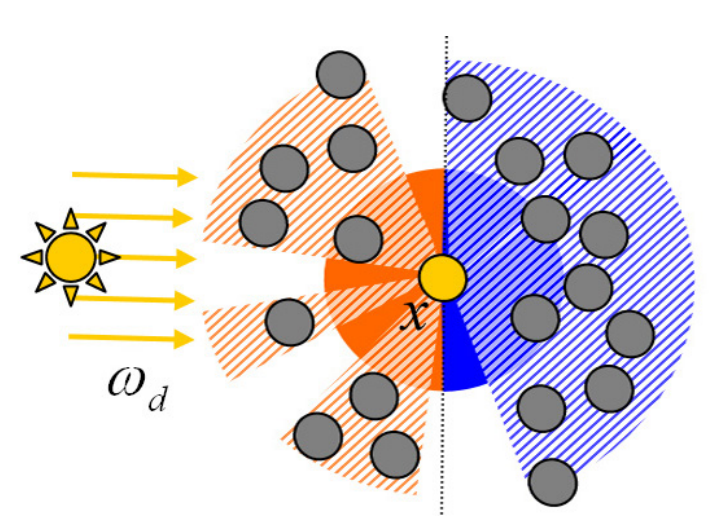
\includegraphics[scale=0.2]{relatedwork/dualscattering_df.png}
\end{center}
\caption{This picture shows the cross section of a hair cluster. The factor $d_f$ is a tweaking variable to account for the portion of multiple scattered radiance reaching the point $x$. The orange region shows the forward scattering contribution. It can be seen that the light could have direct vision with point $x$ in which case there is no multiple scattered radiance. $d_f$ accounts for this fact. If $d_f$ is 1, then it is assumed that point $x$ is fully covered by hair strands as seen from the light direction. The same applies for the backward scattering attenuation factor $d_b$ (blue region). Usually both $d_f$ and $d_b$ are constant for the full model and set to 0.7.}
\label{fig_df}
\end{figure}


$a_f(\theta_d^k)$ is the average forward scattering attenuation at the $k$-th scattering event, which is computed in a precomputation step by integrating over all possible directions in the hemisphere and averaging the amount of forward scattered radiance. See the dual scattering method for more details~\cite{zinke} or the efficient implementation of the dual scattering model in RenderMan by Sadeghi and Tamstorf~\cite{sadeghi} for a more hands on approach.

In this work, a simplification is used by usng a constant orientation for all $k$ scattering events, under the assumption that we are dealing with human hair fibers that are locally similar in orientation. This means equation~\ref{dualscattering_Tf} can be simplified to the following equation.

\begin{equation}
T_f(x, \omega_d) = d_f(x, \omega_d) a_f(\theta_d)^n
\label{forwardscattering}
\end{equation}

\subsubsection{Forward Scattering Spread}

The spread function approximates the final angular distribution of front scattering light to find the probability of radiance coming to the point $x$ from direction $\omega_i$~\cite{zinke}. Because of the wide azimuthal scattering property of hair fibers, front scattered radiance quickly becomes isotropic in the azimuthal direction after only a few scattering events. For longitudinal scattering front scattered light is still anisotropic. The spread function is therefore split up into an isotropic azimuthal component ($1/\pi$) and an anisotropic longitudinal component described by a gaussian function $g$.

\begin{equation}
\label{dualscattering_Sf}
S_f(x, \omega_d, \omega_i) = \frac{s_f(\phi_d, \phi_i)}{\cos \theta_d} g(\theta_d + \theta_i, \sigma_f^2(x, \omega_d))
\end{equation}

where $s_f$ is $1/\pi$ for forward scattering directions and zero for backward scattering. $\sigma_f^2(x, \omega_d$ is the total variance of forward scattering in the longitudinal direction. This is defined by the Marschner model as the squared standard deviation $\beta^2$ and is dependent on the longitudinal angle. Simplifying again by taking a constant $\theta_d$ gives us a single multiplication of number of hair strands multiplied by the longitudinal variance.

\begin{equation}
\sigma_f^2(x, \omega_d) = \sum_{k=1}^{n} \beta_f^2(\theta_d^k) \approx n \cdot \beta_f^2(\theta_d)
\end{equation}


\subsection{Local Multiple Scattering}

The local multiple scattering function $\Psi^L$ accounts for the multiple scattering events within the neighborhood of the point $x$. Since light paths that go through only forward scattering are included in the global multiple scattering function, light paths of the local multiple scattering function must include at least one backward scattering.

Because of backward scattering, the local multiple scattering is mostly smooth with subtle changes over the hair volume~\cite{zinke}.

The dual scattering model the local multiple scattering and the BCSDF of the hair fibers, approximating the result with a density factor $d_b$ and backscattering function.

\begin{equation}
\Psi(x, \omega_d, \omega_i) f_s(\omega_i, \omega_o) \approx d_b(x, \omega_d) f_{\textnormal{back}}(\omega_i, \omega_o)
\end{equation}

The density factor $d_b$ is a constant in the range $[0, 1]$, usually set to 0.7 approximating the density of the hair volume. The denser the hair, the stronger the backscattering event contributes to the result.

The backscattering is approximated with a material function $f_back$

\begin{equation}
f_{\textnormal{back}}(\omega_i, \omega_o) = \frac{2}{\cos \theta_d}A_b(\theta_d) S_b(\omega_i, \omega_o)
\end{equation}

\subsubsection{Average Backscattering Attenuation}

The average backscattering attenuation takes into account the attenuation in the local neighborhood of a point $x$. Since the global multiple scattering component already takes into account the forward scattering (meaning no backscatter events), we only need to deal with at least 1 backscatter event. Light coming from a light source, passing through the fiber at point $x$, needs an odd number of backscattering events for light to travel back to point $x$. The even number of backscattering events are ignored, since they are not directed to point $x$. Also, the dual scattering method ignores the contribution for more than three backscattering events, because their contribution becomes negligible low to the rendering result. 

If we denote $a_b(\theta_d)$ as the average backscattering attenuation and $a_f(\theta_d)$ as the average forward scattering attenuation (described in the previous section), then the average backscattering for a single backscattering event $A_1$ can be computed as the attenuation of a single backscatter event, multiplied by the sum of the infinite series of forward scattering attenuations. The same holds for the average backscattering attenuation for three backscattering events $A_3$, but now the possible paths are not a single sum anymore, but multiple sums to obtain the permutation of possible paths, dependent on where the backscattering event occurs in the sequence of forward scattering attenuations.

\begin{align}
A_1(\theta_d) &= a_b \sum_{i=1}^{\infty} a_f^{2i} = \frac{a_b a_f^2}{1 - a_f^2} \\
A_3(\theta_d) &= a_b^3 \sum_{i=1}^{\infty}  \sum_{j=0}^{i-1} \sum_{k=j+1}^{\infty} a_f^{2(i-j-1+k)} = \frac{a_b^3 a_f^2}{(1 - a_f^2)^3} \\
A_b(\theta_d) = A_1(\theta_d) + A_3(\theta_d)
\end{align}

where $A_b$ is the average backscattering attenuation for 1 and 3 backscattering events. Figure~\ref{avg_backscatter_attenuation} provides a graphics representation of the backscattering events and how they are directed with respect to position $x$.

(picture here)

\subsubsection{Average Backscattering Spread}

The average backscattering spread takes into account the loss of intensity, due to spreading of the light after backscattering events occur. This is similar to forward scattering events. The dual scattering method~\cite{zinke} presents the average backscattering spread $S_b(\omega_i, \omega_o)$ as

\begin{equation}
S_b(\omega_i, \omega_o) = \frac{s_b(\phi_i, \phi_o)}{\cos \theta} g(\theta_o + \theta_i - \Delta_b(\theta_d), \sigma_b^2(\theta_d)
\end{equation}

where $s_b$ equals $1/\pi$ for backward scattering directions and zero for forward scattering, $\Delta_b(\theta_d)$ is the average longitudinal shift caused by the scattering events.

The spread is modeled as a single gaussian function. It is important to notice that $\Delta_b$ represents the average mean and $\sigma^2$ represents the average variance, thereby taking into account the multitude of possible forward and backward scattering events.

The average longitudinal shift $\Delta_b$ and average longitudinal standard deviation $\sigma_b$ for backscattering can be precomputed by averaging over all directions. See the dual scattering method~\cite{zinke} for more details and ~\cite{sadeghi} for a more hands on approach.









\chapter{Approach}

In this thesis the contribution comes from comparing the results for dual scattering method between uniform sampling and the multiple importance sampling strategy by d'Eon et al.~\ref{deon-IS}. This importance sampling strategy has been developed for a hair rendering model by d'Eon and Marschner~\ref{deon}. This model is a continuation of the Marschner model in this paper, where they managed to make the model more efficient by removing the root-solving process (explain better).

First of all a comparison is made by comparing the visual appearance of the image. Is the result obtained with importance sampling looking appropriate for different scenarios, such as when the model is backlit or frontlit, or when the amount of reflection is high. This comparison is rather subjective and to feeling, so we need another way to measure the performance between uniform and importance sampling.

Two ways to evaluate the performance between uniform and importance sampling is by using the variance compared to ground truth and the variance compared to an increasing amount of pixels per samples.

It is important to only compute the variance for the hair volume and not for the background image. This could otherwise give us a false sense of conversion if the hair model covers only a small region of the image. To prevent this from happening, only a specific rectangular region of the image is taken into account that is fully covered by the hair model. The variance is then only computed for this specific region. Figure~\ref{variance-for-region} explains the concept in a graphical way.

(add picture)

\section{Importance sampling for dual scattering method}

In this section I will describe the workings of the physically based importance sampling strategy and how it is applied to the Dual scattering method. The importance sampling strategy is proposed by d'Eon et al.~\cite{eon2013} for the energy conserving improvement of the Marschner model.~\cite{eon2011}.

The usual question with importance sampling is to find an incoming light direction $\omega_i$, given an outgoing direction $\omega_o$. The simple solution, will be to just randomly choose directions and integrate the result. As has been explained in section~\ref{section_importance_sampling} faster convergence can be obtained by specifically selecting an orientation that has more effect on the contributed result.

For implementation purposes PBRT is used, which is an open source physics based ray-tracing framework. In general there are two situations that need to be handled when implementing an importance sampling strategy.

\begin{itemize}
\item Given an outgoing direction $\omega_o$, sample an incident direction $\omega_i$ according to the probability distribution that ideally should be close fit to the shape of the response of the hair rendering model. Besides the incident direction $\omega_i$, also the corresponding PDF should be computed.
\item Given two directions $\omega_i$ and $\omega_o$, what is the probability of sampling $\omega_i$, given $\omega_o$. This is similar to the previous point, except that the output is now only a PDF value.
\end{itemize}

In equation~\ref{marschner_model_scatterfunction} the scattering function for the Marschner model is given. The method by d'Eon et al.~\cite{eon2011} simplifies the equation so that the longitudinal scattering function $M$ is only dependent on longitudinal angles and the azimuthal scattering function $N$ is only dependent on the azimuthal angles. Also the inclination dependent factors, such as the $\cos^2 \theta_d$ term present in the Marschner model are included in the $M_p$ term. This leads to the following equation:

\begin{equation}
S_p(\omega_i, \omega_r) = M_p(\theta_i, \theta_o) N_p(\theta_i, \theta_o, \phi)
\end{equation}

\subsection{Strategy outline}

The idea behind the importance sampling strategy of d'Eon et al.~\cite{eon2013} is to seperate the importance sampling for the longitudinal scattering function and for the azimuthal scattering function. The basic outline of the strategy is as follows.

\begin{itemize}
\item Select a lobe $p \in \{ \textnormal{R}, \textnormal{TT}, \textnormal{TRT} \}$ dependent on the relative contribution of energy reflected. This depends on the Fresnel equation and the absorption coefficient $\sigma$.
\item Given a selected lobe $p$, compute the longitudinal direction by sampling the longitudinal scattering function $M_p$.
\item An outgoing direction $\omega_o$ is given, so we know the spherical angles $\theta_o$ and $\phi_o$.
\item Choose a random offset $h \in [-1, 1]$ along the fiber cross section.
\end{itemize}

The first things that has to be done is lobe selection.

\subsection{Lobe selection}
\label{sec_lobe_selection}

When importance sampling incident directions, we want to take into account the relative contribution of the different lobes in the model. For example, the R component has a stronger influence when viewing hairs from glancing angles compared to the other reflection modes. Hair strands that are backlit do have more contribution from the TT component. It is important to take this into account, because for importance sampling we prefer to sample directions that have more impact on the rendered result than just random sampling.

d'Eon et al.~\cite{eon2013} proposes a way to select lobes by taking into account the attenuations through a smooth, ideally specular fiber $A_{\textnormal{spec}}(p, h)$. The strategy is to first select a random cross-section offset $h = 2\xi_h - 1$,  where $\xi_h \in [0, 1)$ is a uniformly distributed random number. Once the random cross-section offset is known, we can compute the relative contributions for each of the scattering modes.

\begin{align}
A_{\textnormal{spec}}(0, h) &= F(\eta, \gamma_i) \\
A_{\textnormal{spec}}(1, h) &= (1 - F(\eta, \gamma_i))^2 \, T(\sigma_a, h) \\
A_{\textnormal{spec}}(2, h) &= (1 - F(\eta, \gamma_i))^2 \, F(\frac{1}{\eta}, \gamma_t) \, T(\sigma_a, h)^2
\end{align}

These values describe the amount of energy transmitted through or reflected against hair fibers for each of the scattering modes. We do not yet take into account rough fibers, so all energy is concentrated in the specular direction. To sample a lobe, these absolute values should be related to the sum of energy reflected to find the relative weights $w_p$.

\begin{align}
w_{\textnormal{R}} &= \frac{A_{\textnormal{spec}}(0, \gamma_i)}{\sum_p A_{\textnormal{spec}}(p, \gamma_i)} \\
w_{\textnormal{TT}} &= \frac{A_{\textnormal{spec}}(1, \gamma_i)}{\sum_p A_{\textnormal{spec}}(p, \gamma_i)} \\
w_{\textnormal{TRT}} &= \frac{A_{\textnormal{spec}}(2, \gamma_i)}{\sum_p A_{\textnormal{spec}}(p, \gamma_i)}
\end{align}

with the relative weights a lobe can be sampled by taking a random uniform variable $h \in [0, 1)$ and selecting a lobe proportional to the relative attenuation of each component. Once the lobe is known, importance sampling the longitudinal and azimuthal scattering functions become relatively straight forward.

The PDF of the sampling scheme are exactly analogous to evaluation of the model $S$, but with the attenuations $A$ replaced by the selection weights $w_p$~\cite{eon2013}. This makes sense. If the original attenuation factors were to be used, instead of the sample weights, then for all hair models that are not 100 percent transmissive energy will be lost and the PDF will not integrate to 1 anymore. By replacing the attenuations with the sample weights, the PDF is always integrating to 1 irrespective of the hair color.


\subsubsection{Finding the PDF when directions $\omega_o$ and $\omega_i$ are known}

The PBRT framework also requires a function to compute the PDF given two directions $\omega_o$ and $\omega_i$. As stated in the previous section the PDF is analogous to the evaluation of the model $S$, but with the attenuations replaced by the selection weights $w_p$.

The selection weights were determined before by sampling a cross section, giving us the relative contribution per scattering component and thus eventually the relative direction to be sampled. In this case the directions are already known, which means that the relative direction is known. The process is inverse and instead we should now take into account the likelihood of each scattering component to sample the given incident direction.

This is done by solving for roots as has been explained in Marschner related work section~\ref{sec_marschner}. The R and TT components have exactly one root and the TRT component results in one or three roots. This means that any scattering mode could have been selected that would result in the incident direction being sampled. In other words, we need to know the relative probability of a root $h$ to be selected, giving $\omega_i$ as a sampled direction.

This is done in a similar way to sampling a lobe by using the relative attenuation for each of the roots $h$. Since the TRT component could have three roots, it means that this scattering mode actually has three paths to generate the sampled direction. They are summed together to represent the attenuation for the TRT mode. The relative attenuations are then used as the sample weights when evaluating the model $S$ to find the corresponding PDF.


\subsection{Importance sampling the longitudinal M function}
\label{sec_importance_sampling_M}

To importance sample the longitudinal scattering function, we need a way to sample a Gaussian distribution. The essence here is that we are given the outgoing direction $\omega_o = (\theta_o, \phi_o)$ and we need to find the incident longitudinal angle $\theta_i$. The incident $\phi_i$ is determined in the next section (when importance sampling the azimuthal scattering function $M$).

There is a problem with the Gaussian distribution of the Marschner model. First of all it is not energy conserving as has been explained before in section~\ref{marschner_longitudinal_scattering_function}. Part of this can be solved by multiplying the half angle $\theta_h$ by two. Another problem is that especially at glancing angles, part of the energy falls outside of the boundary $\theta \in \{ -\pi/2, \pi/2 \}$, thereby losing energy. This is a problem for importance sampling. When energy is outside of the allowed range, we must somehow compensate this loss of energy in the remaining part of the Gaussian distribution. This is pretty difficult to achieve, at least with the simple normalized gaussian distribution ranging from $\theta \in \{ -\infty, \infty \}$.

d'Eon et al.~\cite{eon2011} proposes a different energy-conserving longitudinal scattering function $M_p$. This function conservatively redistributes reflected radiance amongst directions on the sphere by employing spherical Gaussian convolution. This function is energy conserving and makes sampling a lot easier. The newly used energy conserving scattering function $M$ is as follows:

\begin{equation}
M_p(v, \theta_i, \theta_r) = \frac{\textnormal{csch}(1/v)}{2v} e^{\frac{\sin(-\theta_i)\sin\theta_r}{v}} I_0 \Big [ \frac{\cos(-\theta_i) \cos \theta_r}{v} \Big ]
\end{equation}

where $v$ is the longitudinal scattering variance ($\beta_p^2$) and $I_0$ is the modified Bessel function of the first kind. It is no problem to use a different scattering function to sample from, instead of the Marschner function itself. This is the power of importance sampling, to be able to sample an arbitrary complex function using a simpler and easier to sample function. As long as the function is a good fit, variance will be reduced. More information about the derivation of this function and why it works can be found in the paper by d'Eon et al.~\cite{eon2011}.\\

Sampling a spherical Gaussian can be done with two random numbers $\xi_1$ and $\xi_2$ each within $[0, 1)$. Using the Box-Muller transform gives us a sample for the normalized


\begin{align}
u(\xi_1) &= v \log \Big (e^{1/v} - 2\xi_1 \sinh \frac{1}{v} \Big ) \\
\theta_{\textnormal{cone}, p} &= -\theta_i + \alpha_p\\
\theta' &= \frac{\pi}{2} - \theta_{\textnormal{cone}} \\
\theta_i(\xi_1, \xi_2, v, \theta_{\textnormal{cone}}) &= \nonumber \\
& \arcsin(u(\xi_1) \cos \theta' + \sqrt{1 - u(\xi_1)^2} \cos(2\pi \xi_2) \sin \theta')
\end{align}

At last we end up with the sampled $\theta_i$. The probability of sampling this value is equal to the longitudinal scattering function (assuming it is energy conserving and integrates to 1), therby the PDF is $M \cos^2 \theta_i$.


\subsection{Importance sampling the azimuthal N function}

Importance sampling the azimuthal $N$ function is rather trivial if we know the selected lobe $p$ and the offset $h$ from the scattering cross section (see section~\ref{sec_lobe_selection}). In that case it is a matter of evaluating the relative change in azimuth $\Phi(p, h)$ (see equation~\ref{eq_relative_azimuth_change}), to find the incident azimuth direction $\phi_i$.

\begin{align}
\label{phi_func}
\phi_i^{\textnormal{smooth}} &= \phi_o + \Phi(p, h)
\end{align}

For rough fibers, the relative change in azimuth is offset by a gaussian distributed random variable $g$ with standard deviation 1, multiplied by the width $\beta_p$ corresponding to the selected lobe $p$. Sampling a gaussian distribution can be performed using the Box-Muller transform, that takes two random numbers in the range $[0, 1)$ and samples the normalized gaussian distribution. The direction $\phi_i$ to be importance sampled can thus be found as follows:

\begin{align}
\phi_i &= \phi_o + \Phi(p, h) + g | \beta_p | 
\end{align}

Take into account that the spherical direction wraps around in the range $\{ -\pi, \pi \}$.

\section{The voxel grid}

The dual scattering method proposes different ways to gather global illumination needed for the global multiple scattering component. Among those are ray shooting and forward scattering maps, as explained in Zinke et al.~\cite{zinke}:

\begin{itemize}
\item Ray shooting is the simplest implementation of the global multiple scattering function. To find the forward scattering transmittance and spread at point $x$ due to illumination from direction $\omega_d$, a ray from $x$ is shot in the direction $\omega_d$. If there is no intersection, the direct illumination fraction is set to one. If there is an intersection, then all intersections along the ray are taken into account to compute the transmittance $T_f$ and spread $S_f$ as described by equations~\ref{dualscattering_Tf} and ~\ref{dualscattering_Sf}. Multiple rays per pixel are needed to smooth the results.

\item Forward scattering maps. This is a two pass approach. Each voxel in this grid keeps $T_f$ and $\sigma_f^2$ values along the ray. The values of each voxel are determined by the average of the values along the rays that intersect with the voxel. In the second pass hair geometry is rendered and the global multiple scattering values are found by using linear interpolation from the voxel grid.
\end{itemize}

The implementation in this thesis uses a combination of the above approaches. In this thesis a voxel grid is used together with a two pass approach. The first pass is the voxel grid generation process and the second pass is during rendering when the transmittance and spread values are determined. 

Each hair fiber is represented as a collection of curve segments, where each curve segment is made up of a collection of three dimensional points. In the generation pass, curve segments are stepped through by small increments, thereby linearly interpolating between consecutive points of the curve segment. Each step represents a specific distance. This distance is simply the distance between the current step position and the previous step position. At every step increment the corresponding voxel grid cell is updated with the distance the step is representing. After processing all curve segments, the voxel grid will consist of voxel cells containing the accumulated distances. By relating the accumulated sum of distances with the voxel cell volume, the density of the voxel cell is obtained. The orientations of the individual hair fibers are ignored in the generation process. 

In the rendering pass, the voxel grid is used to find the amount of global multiple scattering at point $x$ from direction $\omega_d$. This is done by integrating from position $x$ in direction $\omega_d$ up to the light position (for an area light) or up to a specifioc limit (in case of directional lights). At each step along the ray, the density is obtained and accumulated so that in the end the complete density is obtained which is treated as the number of hair strands between the light source and the position $x$.

The orientation of the point being shaded is used to compute the spread of light. The orientation is kept constant for all the fibers that are in between point $x$ and the light source. This is a simplification. The reason I chose for this simplification is that hair fibers are usually similar in orientation in the local neighbourhood. Also it makes the voxel generation process less complex. For more realistic behavior that is applicable to more complex hair models, the orientations of the fibers should be taken into account.

There is one edge-case worth mentioning. Hair fibers observed at the boundary of the hair volume, which are directly lit by a light source should have a direct illumination fraction set to 1. However, since this hair fiber is using the density value from the voxel cell, this gives wrong result for directly illuminated hair fibers. To prevent this from happening a shadow ray is traced to check whether the fiber is in shadow. If the fiber is in shadow, the density value of the voxel grid is used and integration happens as described. If the fiber is directly lit by the light source, then the voxel grid is ignored and a direct illumination is set to 1.

For the voxel grid I made use of the openvdb library. To smoothen the density values I used a box sampler to smooth out the sampled density values from the voxel grid. The box sampler trilinearly interpolates samples taken from the voxel grid.

\section{Evaluation against ground truth}

Uniform sampling is the least error prone sampling method that does not need any knowledge about the mathematical model being used. Therefore it is useful to be used for generating the ground truth. The ground truth can be defined as the result obtained by rendering the dual scattering method with uniform sampling by taking a very high amount of samples per pixel for which we can assume that conversion has been reached (for example 1024 samples per pixel).  Any sampling strategy should eventually converge to the same result. We do expect that the importance sampling strategy is converging faster to the ground truth compared to uniform sampling.


\section{Evaluating the conversion rate in terms of variance}

Another way to evaluate the results is to express the variance of the sampling strategy with results of the same sampling strategy, but by using different pixels per sample. By comparing the variance between consecutive results for 1, 2, 4, 8, etc. pixels per samples, we can compute the relative variance as we increase the pixels per samples. You would expect that at some point conversion has been reached. Conversion can be defined as the first image (by increasing the samples per pixel) for which comparing the variance with the previous result is below a threshold variance. We would expect that importance sampling converges faster than uniform sampling.


\chapter{Results}

\section{Hair blocks with different density}

As an indication to see the effects of using the voxel grid. The following images show.
Renderings of cubes with different densities. The left cube is less dense than the right cube. If the cube has a higher density (e.g. more hairs), then more light is scattered around through the model, leading to a darker appearance as you view deeper in the cube.

\begin{figure}[h]
\begin{center}
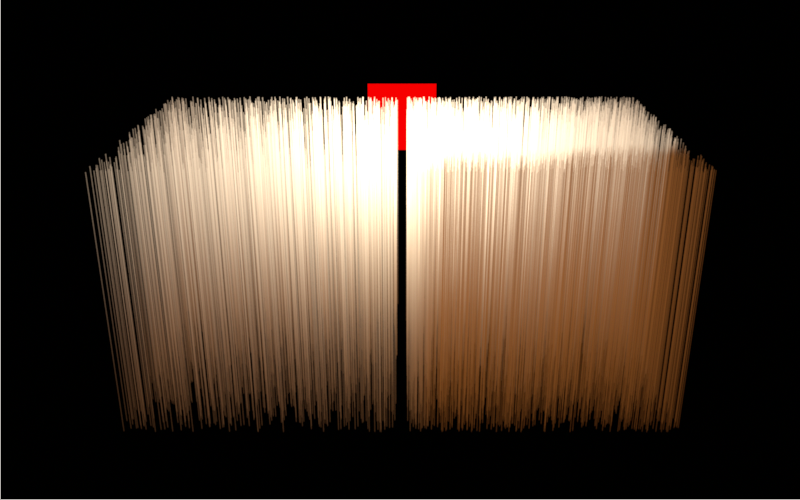
\includegraphics[scale=0.35]{images/dualblock/dualblock_1500_3000_.png} 
\label{dualblock_results}
\caption{Left hair block contains 1500 hairs, versus the right hair block, that contains 3000 hairs.}

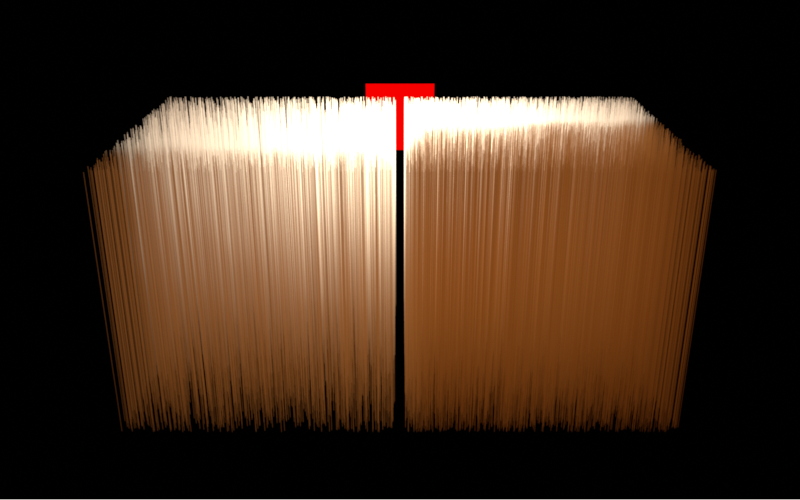
\includegraphics[scale=0.35]{images/dualblock/dualblock_3000_6000_.png}
\label{dualblock_results}
\caption{Left hair block contains 3000 hairs, versus the right hair block, that contains 6000 hairs.}

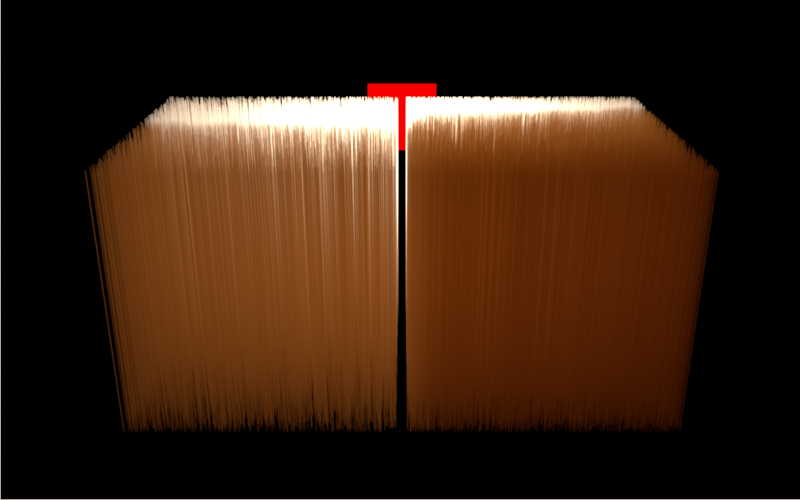
\includegraphics[scale=0.35]{images/dualblock/dualblock_6000_12000_.png}
\caption{Left hair block contains 6000 hairs, versus the right hair block, that contains 12000 hairs.}
\end{center}
\end{figure}


The cubes are rendered with Pixar's Renderman. The size of cubes are \textsc{5x5x5} and are placed on the horizontal plane at \textsc{y = 0}.


\section{Cornwell Scene}

The following images show the effects of the dual scattering algorithm for the well-known cornwell scene. The scene consists of 4 walls: a red wall to the left, a green wall to the right, a gray wall in front and a gray wall behind the camera. The wall behind the camera influences the scene, due to scattered light that reflects back into the visible part of the scene. The red diffuse sphere is present as a reference sphere.

\begin{figure}[h]
\begin{center}
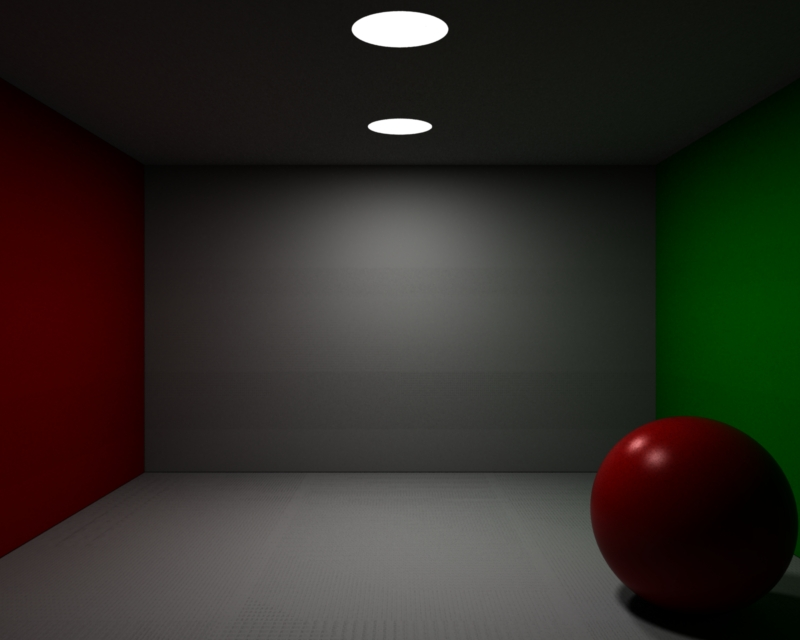
\includegraphics[scale=0.35]{images/scenes/cornwell_empty.jpg}
\label{cornwell_empty}
\caption{Cornwell reference scene without the hair block.}
\end{center}
\end{figure}

\begin{figure}[h]
\begin{center}
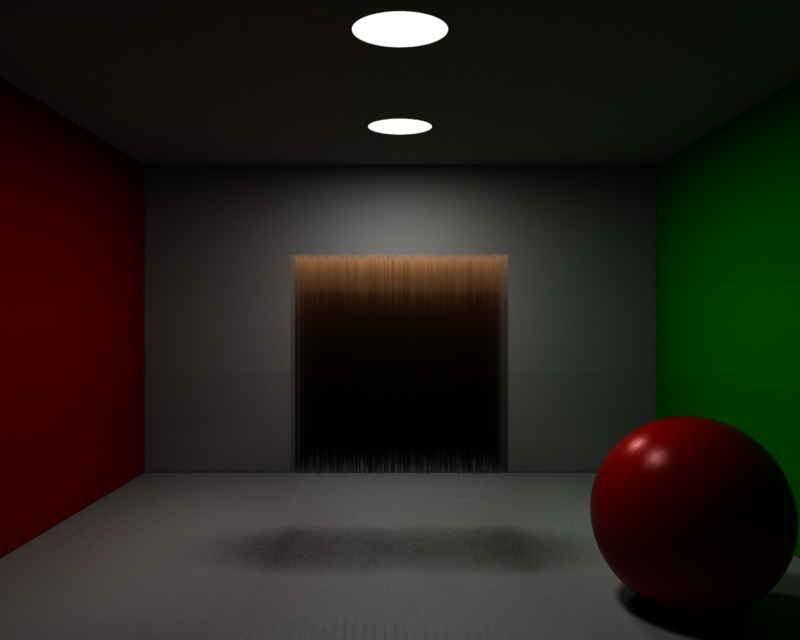
\includegraphics[scale=0.35]{images/scenes/cornwell_uniform.jpg}
\label{cornwell_empty}
\caption{Cornwell reference scene with a uniformly sampled hair block block.}
\end{center}
\end{figure}



\section{Evaluation Strategy}

To evaluate the multiple importance sampling strategy of the dual scattering approximation, we need to render different types of scenes to be able to see that the importance sampling strategy is more efficient that the standard dual scattering approximation. By taking a fixed number of samples for the integration, we expect that the importance sampling strategy will be equally fast in terms of computation speed compared to the non-importance sampling variant. However, the importance sampling strategy should generate an image that is less noisy than the standard dual scattering approximation algorithm using the same number of samples. 



\chapter{Conclusion}

\chapter{Appendix}

\bibliography{thesis}
\bibliographystyle{plain}

\end{document}